\chapter[Philidor~4]{\textit{Philidor~4} : Conception, architecture et analyse}

\textit{Philidor~4} ne s'est pas construite ex nihilo. Elle hérite de trente années d'accumulation de données, de choix techniques antérieurs et de pratiques documentaires qui se sont sédimentées au fil du temps. Comprendre cette base dans sa configuration actuelle nécessite donc de retracer sa genèse, d'analyser ses choix architecturaux et d'évaluer ses performances du point de vue de l'utilisateur final.

Ce chapitre propose une analyse à trois niveaux de la base \textit{Philidor~4}. Il retrace d'abord la genèse du projet, en montrant comment la migration depuis \textit{Philidor III} a été l'occasion de repenser fondamentalement l'architecture des données. Il examine les acteurs impliqués dans cette refonte et les défis qu'ils ont dû relever : consolidation de données hétérogènes, restructuration des relations entre entités, modernisation des interfaces.

Il analyse ensuite l'architecture modulaire retenue, organisée autour de quatre entités principales (\textsc{Source}, \textsc{Œuvre}, \textsc{Événement}, \textsc{Personne}). Cette structure, ambitieuse sur le plan conceptuel, révèle à l'usage certaines complexités qui impactent l'expérience utilisateur. L'analyse quantitative de la répartition des données entre les différentes sous-bases éclaire les usages effectifs de l'outil et révèle certains déséquilibres.

Enfin, le chapitre évalue les fonctionnalités offertes par l'interface actuelle : moteur de recherche, système de navigation, qualité de l'affichage des notices. Cette analyse ergonomique, nourrie par l'observation des pratiques d'utilisateurs réels, identifie les points forts de l'outil mais aussi ses limites en termes d'\gls{accessibilite} et d'intuitivité. Elle pose les bases de la réflexion sur les alternatives éditoriales développées dans le chapitre suivant.

\section{Une entreprise collective : genèse et conception du projet \textit{Philidor~4}}

La refonte de \textit{Philidor} vers sa quatrième version s'inscrit dans un contexte de remise en question globale des outils numériques du \gls{cmbv} au milieu des années 2010. Cette section retrace la genèse de ce projet ambitieux, depuis l'identification des limites de \textit{Philidor III} jusqu'à la définition du cahier des charges de la nouvelle version. Elle présente les différents acteurs impliqués dans cette conception --- équipes techniques, chercheurs, responsables institutionnels --- et analyse comment leurs expertises complémentaires ont façonné les orientations du projet. L'examen des étapes de conception et de migration révèle les défis considérables posés par la consolidation de données accumulées sur trois décennies, ainsi que les arbitrages nécessaires entre continuité et innovation.

\subsection{Contexte et motivations du projet}

\subsubsection{Obsolescence technique et urgence patrimoniale}

Le projet de création de la base de données \textit{Philidor~4} s'inscrit dans une volonté de sauvegarde et de valorisation d'un patrimoine documentaire accumulé pendant près d'un quart de siècle au sein du \gls{cmbv}\footcite{BaseDonneesPHILIDOR42024}. Comme nous l'avons vu précédemment, entre 1995 et 2020, des dizaines de milliers de notices ont été produites dans le cadre de projets de recherche, d'activités éditoriales ou d'enquêtes scientifiques. Ces données étaient jusqu'alors dispersées dans une multitude de supports techniques devenus obsolètes.

Environ 170 bases distinctes avaient été créées sous les systèmes JLB-DOC puis JLB-NET. Ce système avait progressivement montré ses limites. On note notamment une désuétude technologique due au fait que la licence du \gls{cmbv} n'est plus maintenue\footcite{laurentguilloRapportMigrationAnciennes2022}. Cette obsolescence créait une situation d'urgence : le risque de perte définitive de données scientifiques précieuses s'accroissait avec chaque mise à jour des systèmes d'exploitation.

\subsubsection{Inadéquation aux exigences contemporaines}

De plus, ce système ne permet pas de répondre aux exigences actuelles en matière d'\gls{interoperabilite} et de structuration des données. Les normes du \gls{web-semantique}, les protocoles d'échange standardisés et les formats de métadonnées modernes étaient inaccessibles depuis l'architecture JLB, créant un isolement croissant de la ressource dans l'écosystème numérique patrimonial\footcite{laurentguilloRapportMigrationAnciennes2022}. Les nouvelles versions de JLB aurait pu permettre de répondre à ses exigences. Or, une migration vers la version la plus récente de ce système aurait été trop complexe et très coûteuse.

En parallèle, \textit{eZ Publish}, sur lequel reposaient certains développements plus récents, était lui aussi en cours de démantèlement, en raison de l'arrêt de son support et des difficultés techniques rencontrées dans sa maintenance\footcite{laurentguilloRapportMigrationAnciennes2022}. Ces deux systèmes n'étaient plus en mesure de garantir une \gls{accessibilite} pérenne aux données ni de permettre leur exploitation scientifique dans des conditions satisfaisantes.

\subsubsection{Fragmentation des ressources}

À ces bases s'ajoutaient quelques fichiers Excel utilisés pour des projets ponctuels\footcite{laurentguilloRapportMigrationAnciennes2022}. Cette multitude de supports techniques rendait la consultation des données extrêmement complexe, voire inaccessible dans certains cas, en particulier pour les chercheurs extérieurs ou les nouveaux collaborateurs. La fragmentation créait également des risques de redondance et d'incohérence : une même œuvre ou source pouvait être décrite différemment selon les projets, sans mécanisme de contrôle ou de consolidation.

Ainsi, la genèse du projet repose sur une nécessité de consolidation et d'unification, mais aussi sur une ambition de modernisation qui dépasse la simple migration technique.

\subsubsection{Objectifs stratégiques du projet}

Le projet \textit{Philidor~4} visait donc deux objectifs principaux. D'une part, récupérer et préserver ce patrimoine informationnel menacé par l'obsolescence des outils techniques, afin d'éviter la perte irréversible d'années de travail. Cette dimension patrimoniale constituait l'urgence première : sauver l'existant avant qu'il ne devienne définitivement inaccessible.

D'autre part, offrir un environnement de consultation cohérent, structuré et performant, permet des recherches transversales à partir de critères multiples\footcite{laurentguilloRapportMigrationAnciennes2022}. Cette ambition dépassait la simple conservation : il s'agissait de transformer un ensemble de ressources isolées en un véritable outil de découverte scientifique.

La fusion des bases était conçue comme un levier pour faire émerger de nouveaux liens entre données autrefois isolées : rapprochements d'incipits, recoupements biographiques ou événements historiques croisés. Cette vision prospective supposait que l'unification technique permettrait l'émergence de nouvelles pratiques de recherche, exploitant la richesse des croisements possibles entre différents types de notices.

\subsection{Acteurs impliqués dans le projet}

\subsubsection{Direction scientifique et conception}

Ce projet de grande ampleur a mobilisé plusieurs acteurs aux compétences complémentaires. Le travail de conception et de migration a été initié par Laurent Guillo, alors responsable des données numériques au \gls{cmbv}\footcite{BaseDonneesPHILIDOR42024}. Chercheur associé au Centre d'Études Supérieures de la Renaissance (\gls{cesr} — \gls{cnrs}/Université de Tours), spécialiste de la bibliographie matérielle et de l'histoire de l'édition musicale\footcite{GuilloLaurentCESR}, il a mis à profit sa double expertise scientifique et documentaire pour concevoir l'architecture générale de la base.

Son parcours, marqué par une connaissance approfondie des sources imprimées et manuscrites de la musique ancienne, a permis d'aborder la migration avec un regard critique sur les structures existantes et sur les exigences d'un outil de recherche pérenne. Cette expertise disciplinaire a permis l'arbitrage entre les différentes logiques de catalogage héritées des projets antérieurs et la définition d'un modèle de données cohérent.

\subsubsection{Développement technique et implémentation}

Il a été appuyé techniquement par Philippe Ravier, informaticien au sein du \gls{cmbv}, qui a assuré le développement des outils de traitement et la structuration des données\footcite{BaseDonneesPHILIDOR42024}. Cette collaboration entre expertise métier et compétence technique garantissait une approche équilibrée, évitant les écueils d'une conception purement informatique ou exclusivement disciplinaire.

Ensemble, ils ont rédigé le rapport de migration, document clé qui trace les principes, les choix techniques et les arbitrages scientifiques à la base de \textit{Philidor~4}\footcite{laurentguilloRapportMigrationAnciennes2022}. Ce document constitue une véritable mémoire du projet, détaillant les solutions retenues face aux difficultés rencontrées et justifiant les compromis nécessaires.

\subsubsection{Prestation externe et expertise spécialisée}

La société ACATUS Informatique a été chargée de la migration technique\footcite{BaseDonneesPHILIDOR42024}. En effet, ACATUS est une société de services numériques, spécialisée dans le développement d'applications, la gestion de bases de données, la cartographie numérique et l'accompagnement de projets dans les domaines des humanités numériques, du patrimoine et de l'environnement\footcite{ACATUSInformatiqueActeur}. Cette spécialisation dans le secteur culturel constituait un atout décisif pour comprendre les enjeux spécifiques de la migration.

Son équipe a travaillé en étroite collaboration avec le \gls{cmbv} afin de garantir la cohérence structurelle et la compatibilité des outils. Le pilotage du projet au sein d'ACATUS a été assuré par Benjamin Cornu en tant que chef de projet\footcite{BaseDonneesPHILIDOR42024}. Cette expertise sectorielle permettait d'éviter les malentendus entre logiques technique et scientifique, fréquents dans ce type de projets interdisciplinaires.

\subsubsection{Coordination et synthèse}

Ensemble, ces différents acteurs ont œuvré à la centralisation et à la rationalisation d'un corpus de données éparpillées, avec l'objectif de construire une base stable, interrogeable et évolutive, capable de soutenir à long terme les activités de recherche, de documentation et de valorisation menées par le \gls{cmbv}. Cette diversité d'expertises constituait à la fois une richesse et un défi : comment faire converger des logiques professionnelles différentes vers un projet commun ?

\subsection{Méthodologie et étapes de migration}

La migration des bases de données anciennes du \gls{cmbv} vers un système unifié s'est déroulée selon une série d'étapes méthodiquement planifiées, entre 2020 et 2024. Cette approche progressive permettait de minimiser les risques de perte de données tout en maintenant une traçabilité complète des opérations.

\subsubsection{Phase préparatoire : archivage et documentation}

Avant toute migration, 94 bases scientifiques identifiées dans JLB (excluant les bases de test, vides ou désuètes) ont été sauvegardées sous double forme \gls{xml} (\textquote{échange JLB-NET} et \textquote{compatible JLB-DOC}) pour garantir la récupération future de toutes les données\footcite{laurentguilloRapportMigrationAnciennes2022}. Cette redondance des formats de sauvegarde constituait une assurance contre les éventuelles incompatibilités ou corruptions.

Chaque archive incluait la structure de la base JLB, des exports en \gls{rtf} ou \gls{pdf}, des documents éclairant la nature de la base, des images ou \gls{pdf} illustratifs, et un bordereau d'archivage\footcite{laurentguilloRapportMigrationAnciennes2022}. Cette documentation exhaustive permettait de reconstituer le contexte scientifique de chaque base, information cruciale pour la migration ultérieure.

Ces archives ont été cataloguées sous la série "ASN-" des archives scientifiques numériques du \gls{cmbv}\footcite{laurentguilloRapportMigrationAnciennes2022}. Cette intégration dans le système d'archivage institutionnel garantit leur conservation à long terme et leur \gls{accessibilite} pour de futurs projets.

\subsubsection{Phase de sélection et préparation}

Un second tri a conduit à sélectionner 70 bases élémentaires ou composites dont le contenu scientifique devait être prioritairement conservé\footcite{laurentguilloRapportMigrationAnciennes2022}. Cette sélection s'appuyait sur des critères de pertinence scientifique, de qualité des données et de complémentarité avec les corpus existants.

Il a été décidé de migrer le contenu de ces 70 bases JLB vers quatre sous-bases MySQL indépendantes dans \textit{Philidor~4} : \textsc{Personne} (PROSOPO), \textsc{Événement} (CHRONO), \textsc{Source} (SOURCES) et \textsc{Œuvre} (ŒUVRES ou FRAGMENTS)\footcite{laurentguilloRapportMigrationAnciennes2022}\footcite{BaseDonneesPHILIDOR42024}. Cette structuration en quatre entités constituait l'innovation majeure du projet, permettant de rationaliser la diversité des anciens catalogues selon une logique conceptuelle unifiée.

Un référentiel de champs commun a été progressivement constitué pour toutes ces sous-bases\footcite{laurentguilloRapportMigrationAnciennes2022}. Cette harmonisation supposait de résoudre les divergences de vocabulaire et de structure entre les différents projets historiques, tout en préservant la richesse descriptive spécifique à chaque domaine.

Pour chaque base JLB, un ou deux intrants (fichiers \gls{xml}) ont été créés, leur qualité a été vérifiée et améliorée manuellement. Ces intrants ont fait l'objet de spécifications de migration avant d'être chargés dans MySQL. La dernière version de chaque intrant a également été archivée\footcite{laurentguilloRapportMigrationAnciennes2022}. Cette double validation — automatique puis manuelle — permettait de détecter et corriger les anomalies avant l'intégration définitive.

\subsubsection{Traitement des sources complémentaires}

Les bases \textit{eZ Publish} déjà migrées depuis JLB vers MySQL ont été ignorées, leurs données ayant été reprises directement de JLB\footcite{laurentguilloRapportMigrationAnciennes2022}. Cette économie d'effort évitait les duplications inutiles tout en maintenant la cohérence des sources.

Cependant, quelques bases \textit{eZ Publish} qui n'existaient que là, comme CHRONO\_BROSSARD, CHRONO\_RAMEAU, et AUDIENCES (renommée ALMANACH), ont été extraites en \gls{xml}, reformatées, nettoyées et chargées dans \textit{Philidor~4}\footcite{laurentguilloRapportMigrationAnciennes2022}. Ces corpus spécialisés apportaient des compléments thématiques précieux qui justifiaient l'effort de récupération.

Deux fichiers Excel (OPERA\_1721\_1791 et REGENCE\_1714\_1724) ont également été reformatés en \gls{xml} et chargés dans la sous-base CHRONO de \textit{Philidor~4}\footcite{laurentguilloRapportMigrationAnciennes2022}. Ces données chronologiques, bien que produites dans des formats rudimentaires, contenaient des informations uniques qu'il était important de préserver et d'intégrer dans l'ensemble.

\subsubsection{Phase finale : consolidation et unification}

Les quatre bases intermédiaires (\textsc{Personne}, \textsc{Événement}, \textsc{Source}, \textsc{Œuvre/Fragment}) ont été rechargées dans une base MySQL unique nommée \textit{Philidor~4}. Cette consolidation finale permettait de bénéficier à la fois de la cohérence structurelle et des possibilités de recherche transversale.

Les noms des projets ont été renommés et simplifiés pour regrouper les données de manière plus logique\footcite{laurentguilloRapportMigrationAnciennes2022}. Cette rationalisation de la nomenclature facilitait la navigation pour les utilisateurs tout en préservant la traçabilité vers les projets originaux.

Le projet de création de \textit{Philidor~4} représente ainsi une étape structurante dans l'histoire numérique du \gls{cmbv}. Elle témoigne d'une prise de conscience institutionnelle de l'importance de traiter les données patrimoniales comme des actifs à préserver et à faire dialoguer, au-delà des cadres techniques qui les ont portées initialement. Cette migration constitue également un modèle méthodologique pour d'autres institutions confrontées aux mêmes défis de préservation et de modernisation de leurs ressources numériques.

\section{Architecture modulaire : quatre sous-bases autonomes}

Le choix d'une architecture modulaire constitue l'innovation majeure de \textit{Philidor~4}. Cette section analyse la logique de structuration retenue, qui distingue quatre entités principales (\textsc{Source}, \textsc{Œuvre}, \textsc{Événement}, \textsc{Personne}) interconnectées par un système de relations complexes. Elle examine les avantages théoriques de cette approche --- flexibilité, évolutivité, cohérence conceptuelle --- mais aussi ses implications pratiques pour les utilisateurs et les gestionnaires de données. L'analyse de la consolidation technique sous MySQL révèle les défis posés par l'unification de bases de données auparavant distinctes. La répartition quantitative des données entre les sous-bases éclaire enfin les usages effectifs de l'outil et révèle certains déséquilibres entre les différents types d'informations.

\subsection{Conception et fondements de l'architecture modulaire}

\subsubsection{Logique ontologique et héritage méthodologique}

La structuration de \textit{Philidor~4} en quatre sous-bases conceptuelles --- \textsc{Source}, \textsc{Œuvre}, \textsc{Événement} et \textsc{Personne} --- répond à une volonté de rationaliser un patrimoine informationnel complexe, hérité de décennies de travail, tout en optimisant l'accès, la pérennité et l'exploitabilité des données. Cette quadripartition reflète les catégories fondamentales de la recherche musicologique : les objets matériels (\textsc{Sources}), les créations artistiques (\textsc{Œuvre}), les faits historiques (\textsc{Événement}) et les acteurs (\textsc{Personne}).

Bien que toutes les notices soient physiquement intégrées dans une unique base (\textit{Philidor~4}), cette division logique constitue un élément central de l'architecture, autant par souci de continuité historique que par nécessité technique et scientifique. Elle permet de maintenir une cohérence conceptuelle tout en facilitant l'évolution future du système.

Cette approche s'inscrit dans la continuité de schémas méthodologiques développés au fil des générations technologiques successives. Le système \textit{Philidor} s'est développé à travers plusieurs environnements (JLB-DOC, JLB-NET, \textit{eZ Publish}), chacun accumulant son propre corpus. Les migrations successives ne prenaient pas toujours en compte l'ensemble des bases existantes tandis que chaque nouveau projet s'insérait sur le système alors en place.

Dès 1997, une organisation en quatre fichiers (\textit{Œuvres}, \textit{Bibliographie}, \textit{Archives} et \textit{Annuaire}) était déjà en usage, et \textit{Philidor~III} avait formalisé les concepts d'\textquote{unité d'objet}, \textquote{unité de personne}, \textquote{unité de temps} et \textquote{unité de lieu}\footcite[Rapport sur le projet Philidor de Jérémie Crublet, juin 2006]{michelbenoitDocumentationTechniqueBibliographique1997}. La structuration retenue dans \textit{Philidor~4} prolonge et affine cette logique, témoignant d'une maturation progressive de la réflexion documentaire au sein de l'institution. Cette continuité conceptuelle facilitait l'appropriation du nouveau système par les utilisateurs habitués aux versions antérieures.

\subsubsection{Avantages fonctionnels de la modularité}

Bien que les notices soient regroupées dans une base unique, chacune est caractérisée par des codes spécifiques (nature, type, etc.) qui permettent un filtrage précis\footcite{laurentguilloRapportMigrationAnciennes2022}. Cette conception préserve les possibilités de recherche ciblée par type d'objet --- par exemple, consulter uniquement les \textsc{Personnes} ou les \textsc{Œuvres} --- tout en rendant possible des rapprochements entre catégories qui, dans les systèmes précédents, auraient nécessité des recherches distinctes\footcite{laurentguilloRapportMigrationAnciennes2022}.

Les utilisateurs bénéficient ainsi d'un accès souple, combinant spécialisation et transversalité. Cette flexibilité répond aux différentes stratégies de recherche : approche focalisée sur un type d'objet spécifique, ou exploration interdisciplinaire croisant plusieurs catégories. La modularité technique sert donc une ambition épistémologique : faciliter l'émergence de nouvelles questions de recherche par le croisement de données auparavant isolées.

Les quatre natures d'objets retenues correspondent aux fondements mêmes de la recherche musicologique conduite par le \gls{cmbv}. Cette distinction catégorielle garantit la continuité des méthodes de travail, tout en offrant un cadre stable pour le développement de nouvelles fonctionnalités de recherche, d'analyse et de diffusion. En somme, la division conceptuelle de \textit{Philidor~4} traduit un équilibre entre héritage et innovation : elle assure la cohérence d'un ensemble documentaire riche et hétérogène, tout en ouvrant la voie à des exploitations scientifiques et techniques élargies.

\subsection{Implémentation technique et défis de consolidation}

\subsubsection{Choix technologique et architecture MySQL}

Dans une logique de modernisation et de rationalisation de son infrastructure numérique, le \gls{cmbv} a entrepris de migrer les anciennes bases de données vers un système unifié reposant sur MySQL. Ce choix a d'abord été motivé par le fait que ce système de gestion de bases de données est libre et largement utilisé\footcite{laurentguilloRapportMigrationAnciennes2022}. Cette popularité garantissait la disponibilité de compétences techniques et la pérennité de la solution à long terme.

MySQL offre également l'avantage d'une compatibilité éprouvée avec les environnements web, facilitant le développement d'interfaces de consultation et d'administration. Sa robustesse et ses performances, validées par de nombreux projets dans le secteur culturel, en font un choix technique rassurant pour un projet de cette ampleur. De plus, MySQL, déjà utilisé au sein du \gls{cmbv} notamment dans les installations Omeka-S, offrait un environnement familier, interopérable et capable de s'inscrire dans une infrastructure normalisée\footcite{laurentguilloRapportMigrationAnciennes2022}.

L'intégration dans l'écosystème technique existant constituait un enjeu crucial : éviter la création d'un nouvel îlot technologique qui aurait reproduit les problèmes de dispersion qu'il s'agissait de résoudre. La compatibilité avec les autres outils en usage au \gls{cmbv} garantissait les possibilités d'évolution future et d'interconnexion avec d'autres ressources.

La base ainsi constituée regroupe l'ensemble des données migrées dans une structure unique, organisée autour des quatre sous-bases principales. Ces ensembles sont chacun interrogeables à l'aide d'un référentiel de champs commun, avec des codes qualifiants permettant de filtrer et de croiser les recherches. Cette harmonisation des vocabulaires de description constituait l'un des défis majeurs de la migration.

Cette structuration a permis de rendre les données plus intelligibles, de corriger des anomalies techniques\footnote{Notamment liées aux jeux de caractères, aux apostrophes ou aux ligatures}, et de simplifier des artifices de mise en page qui compliquaient jusqu'alors la lecture ou l'exploitation scientifique\footcite{laurentguilloRapportMigrationAnciennes2022}. La normalisation des caractères constituait un enjeu technique majeur : les systèmes antérieurs utilisaient des encodages divers, créant des problèmes d'affichage et de recherche. La migration vers UTF-8 garantit désormais une compatibilité universelle et une recherche textuelle fiable, conditions indispensables pour un outil scientifique moderne.

\subsubsection{Gestion des héritages complexes}

Les anciennes pratiques de saisie, issues de projets multiples, avaient généré une forte redondance des notices : une même œuvre ou source pouvait être décrite plusieurs fois dans des contextes différents\footcite{laurentguilloRapportMigrationAnciennes2022}. Cette redondance reflétait la logique de projet qui avait prévalu historiquement, chaque équipe créant ses propres références sans coordination avec les autres initiatives.

Bien que la migration n'ait pas permis d'éliminer entièrement la redondance héritée de l'ancien système, elle a offert une base de travail beaucoup plus cohérente. La structuration en quatre sous-bases ne supprime pas d'emblée cette redondance, mais elle en facilite l'identification et la gestion future, en classant les informations selon leur nature\footcite{laurentguilloRapportMigrationAnciennes2022}. Cependant, en attendant cette identification et gestion future, la persistance de ces redondances peut créer du bruit dans les recherches, générant des résultats multiples pour un même objet.

Les anciens noms de projets, souvent complexes et spécifiques, ont été renommés et regroupés\footcite{laurentguilloRapportMigrationAnciennes2022}, facilitant la lisibilité des jeux de données et la constitution de corpus thématiques plus homogènes. Cette rationalisation de la nomenclature s'accompagnait d'un travail d'harmonisation des vocabulaires de description, nécessaire pour permettre des recherches cohérentes à travers les différents corpus. Les variations terminologiques entre projets étaient nombreuses : un même concept pouvait être désigné par des termes différents selon les équipes et les époques.

La relation \textquote{n,n} entre œuvres et sources était complexe et s'est présentée comme une difficulté majeure. Une source peut contenir plusieurs œuvres, et une œuvre peut être transmise par plusieurs sources, créant un réseau de relations qu'il fallait modéliser et préserver. Les liens complexes qui relient ces objets --- par exemple, entre une \textsc{Source} et l'\textsc{Œuvre} qu'elle transmet, ou entre un \textsc{Événement} et les \textsc{Personnes} qui y participent --- peuvent ainsi être organisés plus efficacement. Cette rationalisation progressive des relations constitue l'un des enjeux à long terme du projet.

Par ailleurs, les liens entre une œuvre et ses fragments, c'est-à-dire des éléments dépouillés, n'étaient pas toujours cohérents et pointaient parfois vers une source au lieu d'une œuvre. Ces liens ont été reconstruits dans la mesure du possible\footcite{laurentguilloRapportMigrationAnciennes2022}.

\subsubsection{Impact et perspectives d'évolution}

Ces ajustements techniques illustrent la tension permanente entre préservation de l'information historique et exigences de normalisation informatique.

En définitive, cette consolidation sous MySQL a marqué une étape décisive dans l'évolution des outils numériques du \gls{cmbv}. Elle a non seulement permis de sauvegarder un patrimoine documentaire précieux, mais aussi d'améliorer considérablement les possibilités de recherche et d'analyse croisée, en ouvrant la voie à des usages scientifiques renouvelés et à une meilleure \gls{interoperabilite} avec les autres systèmes en place.

La base unifiée facilite désormais la maintenance technique, réduit les coûts d'hébergement et de sauvegarde, et simplifie les procédures de mise à jour. Cette rationalisation technique libère des ressources pour le développement de nouvelles fonctionnalités et l'amélioration de l'expérience utilisateur, objectifs qui étaient difficiles à atteindre dans l'ancien contexte de dispersion technologique.

Cette architecture modulaire constitue le socle sur lequel peuvent s'appuyer de futurs développements, qu'ils soient techniques (nouvelles fonctionnalités) ou scientifiques (nouveaux corpus). La flexibilité conceptuelle et technique désormais acquise permet d'envisager des évolutions majeures sans remise en cause fondamentale de la structure, garantissant ainsi la pérennité de l'investissement documentaire et technique réalisé.

\subsection{Répartition quantitative et analyse des contenus}

La base de données \textit{Philidor~4} constitue un patrimoine documentaire considérable du \gls{cmbv}. Cette section présente les principales caractéristiques quantitatives de cette ressource, établies en avril 2022. Ces données révèlent l'ampleur du travail de consolidation réalisé et permettent d'évaluer l'équilibre entre les différents types de contenus.

\subsubsection{Vue d'ensemble : volume et \gls{accessibilite}}

La base \textit{Philidor~4} rassemble un total de \textbf{82~623 notices}\footcite{laurentguilloRapportMigrationAnciennes2022}, dont la répartition en termes d'\gls{accessibilite} révèle une politique d'ouverture privilégiant la diffusion publique des données :

\begin{itemize}
	\item \textbf{90,5~\%} du contenu (soit la majorité des notices) est accessible au public,
	\item \textbf{9,5~\%} du contenu est placé dans une base \textquote{réservée}, nécessitant un accès restreint par mot de passe attribué par le \gls{cmbv}.
\end{itemize}

Cette répartition témoigne d'une volonté institutionnelle de valorisation scientifique, la restriction d'accès ne concernant qu'une minorité de contenus, probablement liés à des projets en cours ou à des questions de droits d'auteur. La prédominance de l'accès libre favorise la visibilité de la ressource et son appropriation par la communauté scientifique.

\subsubsection{Architecture et distribution par entités}

Le tableau~\ref{tab:repartition_sousbases} présente la répartition quantitative des sous-ensembles et révèle des déséquilibres significatifs entre les différentes catégories\footcite{BaseDonneesPHILIDOR42024}.

\begin{table}[htbp]
	\centering
	\caption{Répartition des notices par sous-base dans \textit{Philidor~4}}
	\label{tab:repartition_sousbases}
	\begin{tabular}{lrr}
		\toprule
		\textbf{Sous-base} & \textbf{Nombre de notices} & \textbf{Pourcentage} \\
		\midrule
		Œuvres (FRAGMENTS) & 55~175 & 66,8~\% \\
		Événement (CHRONO) & 10~951 & 13,3~\% \\
		Sources (SOURCES) & 14~247 & 17,2~\% \\
		Personne (PROSOPO) & 2~250 & 2,7~\% \\
		\midrule
		\textbf{Total} & \textbf{82~623} & \textbf{100~\%} \\
		\bottomrule
	\end{tabular}
\end{table}

Cette répartition révèle une concentration marquée sur les œuvres et fragments (plus de la moitié du corpus total), suivie par les événements chronologiques. Cette distribution reflète les orientations historiques du \gls{cmbv}, privilégiant le catalogage des créations musicales et la reconstitution de la vie musicale par l'approche événementielle.

\subsubsection{Analyse de la sous-base Personne (PROSOPO)}

Cette sous-base, la plus modeste avec 2~250 notices, se concentre principalement sur les données issues du projet \enquote{LIONROME V6}, consacré à la description des musiciens romains de la période 1570-1750. Cette spécialisation géographique et chronologique illustre le caractère encore partiel de la couverture \glslink{prosopographie}{prosopographique} de \textit{Philidor~4}.

Le faible volume de cette sous-base contraste avec l'importance des personnes dans la recherche musicologique : compositeurs, interprètes, commanditaires, copistes constituent des acteurs centraux de la vie musicale. Cette sous-représentation s'explique par l'historique des projets du \gls{cmbv}, davantage orientés vers la description des œuvres que vers la prosopographie systématique.

L'objectif idéal d'étendre cette couverture à toutes les personnes référencées dans les autres sous-bases en tant qu'autorité souligne l'ambition de constituer un référentiel \glslink{prosopographie}{prosopographique} exhaustif. Cette évolution transformerait qualitativement la base en permettant des recherches biographiques et relationnelles approfondies.

\subsubsection{Analyse de la sous-base Événement (CHRONO)}

Avec 10~951 notices, cette sous-base constitue le troisième ensemble le plus volumineux\footcite{BaseDonneesPHILIDOR42024}. Elle agrège les données de nombreux projets chronologiques spécialisés. Cette approche événementielle reflète une conception de l'histoire musicale privilégiant la reconstitution de la vie musicale dans sa dimension temporelle et contextuelle.

La prédominance des événements liés à la cour de France (2~883 notices cumulées, soit environ un quart de la sous-base) révèle une focalisation sur l'institution musicale centrale de l'Ancien Régime. Cette concentration géographique et sociale reflète la richesse documentaire des archives royales. On peut également rappeler la vocation première du \gls{cmbv} : \textquote{redonner au Château de Versailles sa musique et à la musique baroque française des XVII\textsuperscript{e} et XVIII\textsuperscript{e} siècles sa grandeur, sa justesse et son style originel}\footcite{CentreMusiqueBaroque}. Avec cet éclairage, cette prédominance devient d'autant plus logique puisque ces études participent par là aux orientations scientifiques du \gls{cmbv}. Les autres corpus (opéras, académies provinciales, chronologies individuelles) apportent des compléments thématiques et géographiques qui nuancent cette centralité parisienne.

La diversité des sources de cette sous-base (presse périodique, archives institutionnelles, reconstitutions chronologiques) témoigne de la variété des approches méthodologiques dans la reconstitution de la vie musicale historique.

\subsubsection{Analyse de la sous-base Sources (SOURCES)}

Cette sous-base rassemble 14~247 notices décrivant diverses sources imprimées et manuscrites. Elle est donc la deuxième la plus importante. Elle comprend notamment les sources de l'air de cour (AIRCOUR), les éditions Ballard (BALLARD), les recueils d'airs sérieux et à boire (RASBSOUR), ainsi que les références du \gls{rism}.

Cette diversité typologique révèle l'ambition de couvrir l'ensemble de la chaîne de transmission musicale, depuis les manuscrits d'auteur jusqu'aux éditions commerciales, en passant par les copies et adaptations. La présence de données \gls{rism} souligne l'inscription de \textit{Philidor~4} dans les réseaux internationaux de catalogage des sources musicales.

\subsubsection{Analyse de la sous-base Œuvres}

Constituant l'ensemble le plus volumineux avec 55~175 notices (66,8~\% du total), cette sous-base regroupe une diversité de catalogues qui reflète la richesse et la complexité du patrimoine musical français. Cette prédominance quantitative témoigne de l'orientation privilégiée du \gls{cmbv} vers la description et l'analyse des créations musicales. La sous-base intègre plusieurs types de contenus complémentaires.

Les catalogues individuels constituent l'épine dorsale de cette sous-base, avec notamment Marc-Antoine Charpentier (2~368 notices), Nicolas Bernier, Lully, Rameau. Ces corpus monographiques permettent des études stylistiques approfondies et facilitent l'identification des œuvres dans les sources historiques. Par ailleurs, les regroupements par genres (cantates, parodies spirituelles, airs de cour) offrent une perspective transversale sur l'évolution des formes musicales. Cette approche typologique complète l'approche monographique en révélant les circulations et influences entre compositeurs. De plus, l'intégration de catalogues déjà publiés (Hitchcock, Agen) témoigne d'une volonté d'exhaustivité et de consolidation de la littérature scientifique existante. Cette récupération de données externes enrichit considérablement les contenus tout en évitant la duplication d'efforts. Enfin, la présence massive de la bibliographie Lachèvre (15~381 notices de poésies) et du fichier Verchaly (5~965 poésies) révèle l'attention portée aux textes littéraires associés à la musique. Cette dimension textuelle enrichit considérablement les possibilités d'analyse interdisciplinaire.

Cette diversité constitue à la fois une richesse et un défi : comment maintenir la cohérence de description face à des objets aussi hétérogènes ? La coexistence de catalogues d'œuvres musicales et de bibliographies poétiques dans la même sous-base pose des questions de modélisation et d'interface qui se répercutent sur l'expérience utilisateur.

\section{Fonctionnalités et ergonomie}

L'évaluation de \textit{Philidor~4} ne peut se limiter à ses aspects techniques ; elle doit également examiner l'expérience concrète des utilisateurs face à l'interface proposée. Cette section analyse les fonctionnalités du moteur de recherche, en évaluant ses potentialités mais aussi ses limites. Elle examine les modalités de navigation proposées, depuis les index alphabétiques jusqu'aux parcours de découverte, en questionnant leur efficacité pour différents types d'usagers. L'analyse de l'affichage des notices révèle quant à elle les enjeux de présentation de l'information. Cette évaluation ergonomique pose les bases de la réflexion sur les alternatives éditoriales développées dans le chapitre suivant.

\subsection{Architecture et fonctionnalités du moteur de recherche}

Les moteurs de recherche sont des outils complexes qui servent de point d'accès principal aux collections en ligne, qu'il s'agisse de bibliothèques numériques ou de bases de données. Leur fonction est d'optimiser la pertinence des résultats de recherche à partir de diverses données.\footcite{bermesMoteursRecherche2007}

\subsubsection{Organisation modulaire de l'interface}

L'interface de recherche de \textit{Philidor~4} s'organise autour d'une architecture modulaire reflétant la structure de la base : quatre onglets donnent accès aux formulaires correspondant aux sous-bases \textsc{Source} (cf. figure \ref{source-onglet}), \textsc{Œuvre}, \textsc{Événement} et \textsc{Personne}. Cette segmentation thématique permet une interrogation ciblée des données selon leur nature.

\begin{figure}[h]
	\caption{Onglet de recherche pour la sous-base \textsc{Source}} \label{source-onglet}
	\centering
	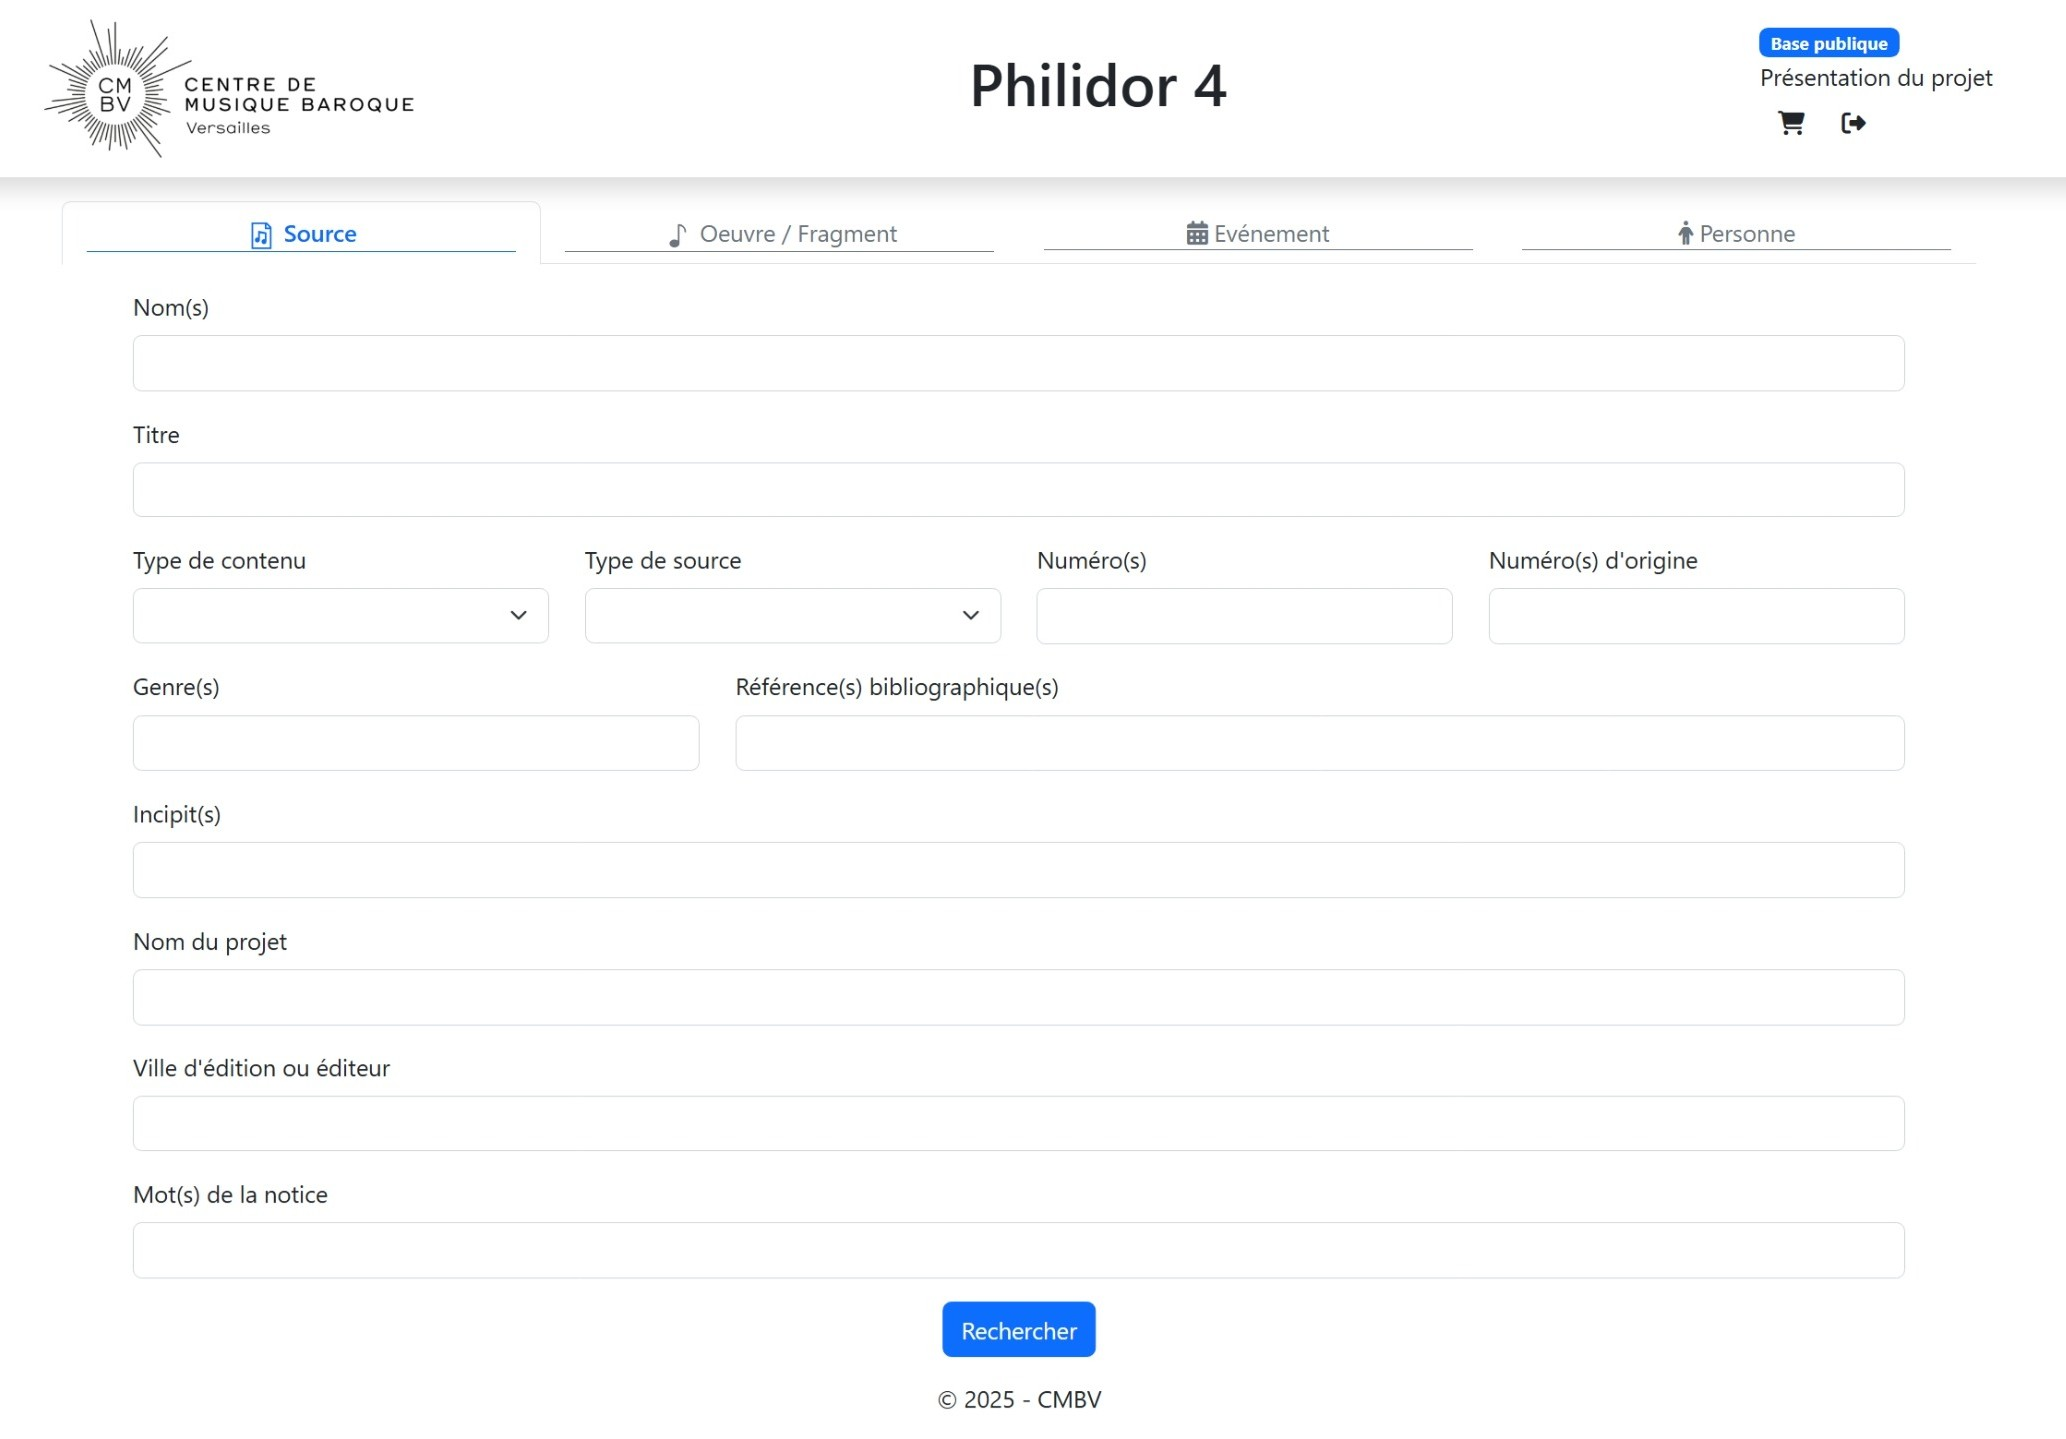
\includegraphics[width=\textwidth]{images/Capture_ecran_onglet_sources_philidor4.jpeg}
\end{figure}

Cette organisation répond à une logique documentaire classique : spécialiser les outils de recherche selon le type d'objet recherché. En effet, les moteurs de recherche sont conçus pour traiter de vastes quantités de données textuelles, hétérogènes et diverses ; certaines solutions sont adaptées à des corpus homogènes comme un domaine ou un type de données en particulier, tandis que les corpus généralistes et multilingues posent des défis plus importants\footcite{bermesMoteursRecherche2007}. Ainsi, l'approche choisi par le \gls{cmbv} préfère diviser pour mieux régner. Ses moteurs de recherche spécialisés présentent l'avantage de proposer des critères adaptés à chaque catégorie, évitant la surcharge cognitive d'un formulaire unique trop complexe. Cependant, elle suppose de la part de l'utilisateur une connaissance préalable de la typologie des contenus et de leur répartition entre sous-bases.

Le moteur de recherche exploite ensuite les données structurées issues des notices\footcite{bermesMoteursRecherche2007} pour renvoyer des résultats correspondant aux critères. Chaque formulaire propose donc des champs spécialisés, certains contraints par des vocabulaires contrôlés (types de contenu, types de source), d'autres permettant la saisie libre. Un mécanisme de restriction par projet, commun à tous les onglets, permet de circonscrire les requêtes selon les corpus disponibles, fonctionnalité particulièrement utile pour les chercheurs travaillant sur des fonds spécifiques.

L'utilisation de guillemets pour délimiter les chaînes exactes dans les champs de titre et d'incipits\footcite{BaseDonneesPHILIDOR42024} révèle une attention portée aux besoins de précision documentaire. Cette fonctionnalité permet de distinguer les recherches approximatives des requêtes exactes.

\subsubsection{Spécificités des sous-bases et adaptations thématiques}

La sous-base \textsc{Œuvre} intègre une fonctionnalité particulière : l'inclusion ou l'exclusion des fragments (éléments dépouillés) via une case à cocher (cf. figure \ref{formulaire_oeuvre}). Cette option révèle la volonté de distinguer les œuvres complètes des extraits, distinction fondamentale en musicologie mais qui pose des défis d'identification dans les résultats, car aucun marquage visuel ne permet de les différencier a posteriori.

\begin{figure}[h]
	\caption{Onglet de recherche pour la sous-base \textsc{Œuvre}} \label{formulaire_oeuvre}
	\centering
	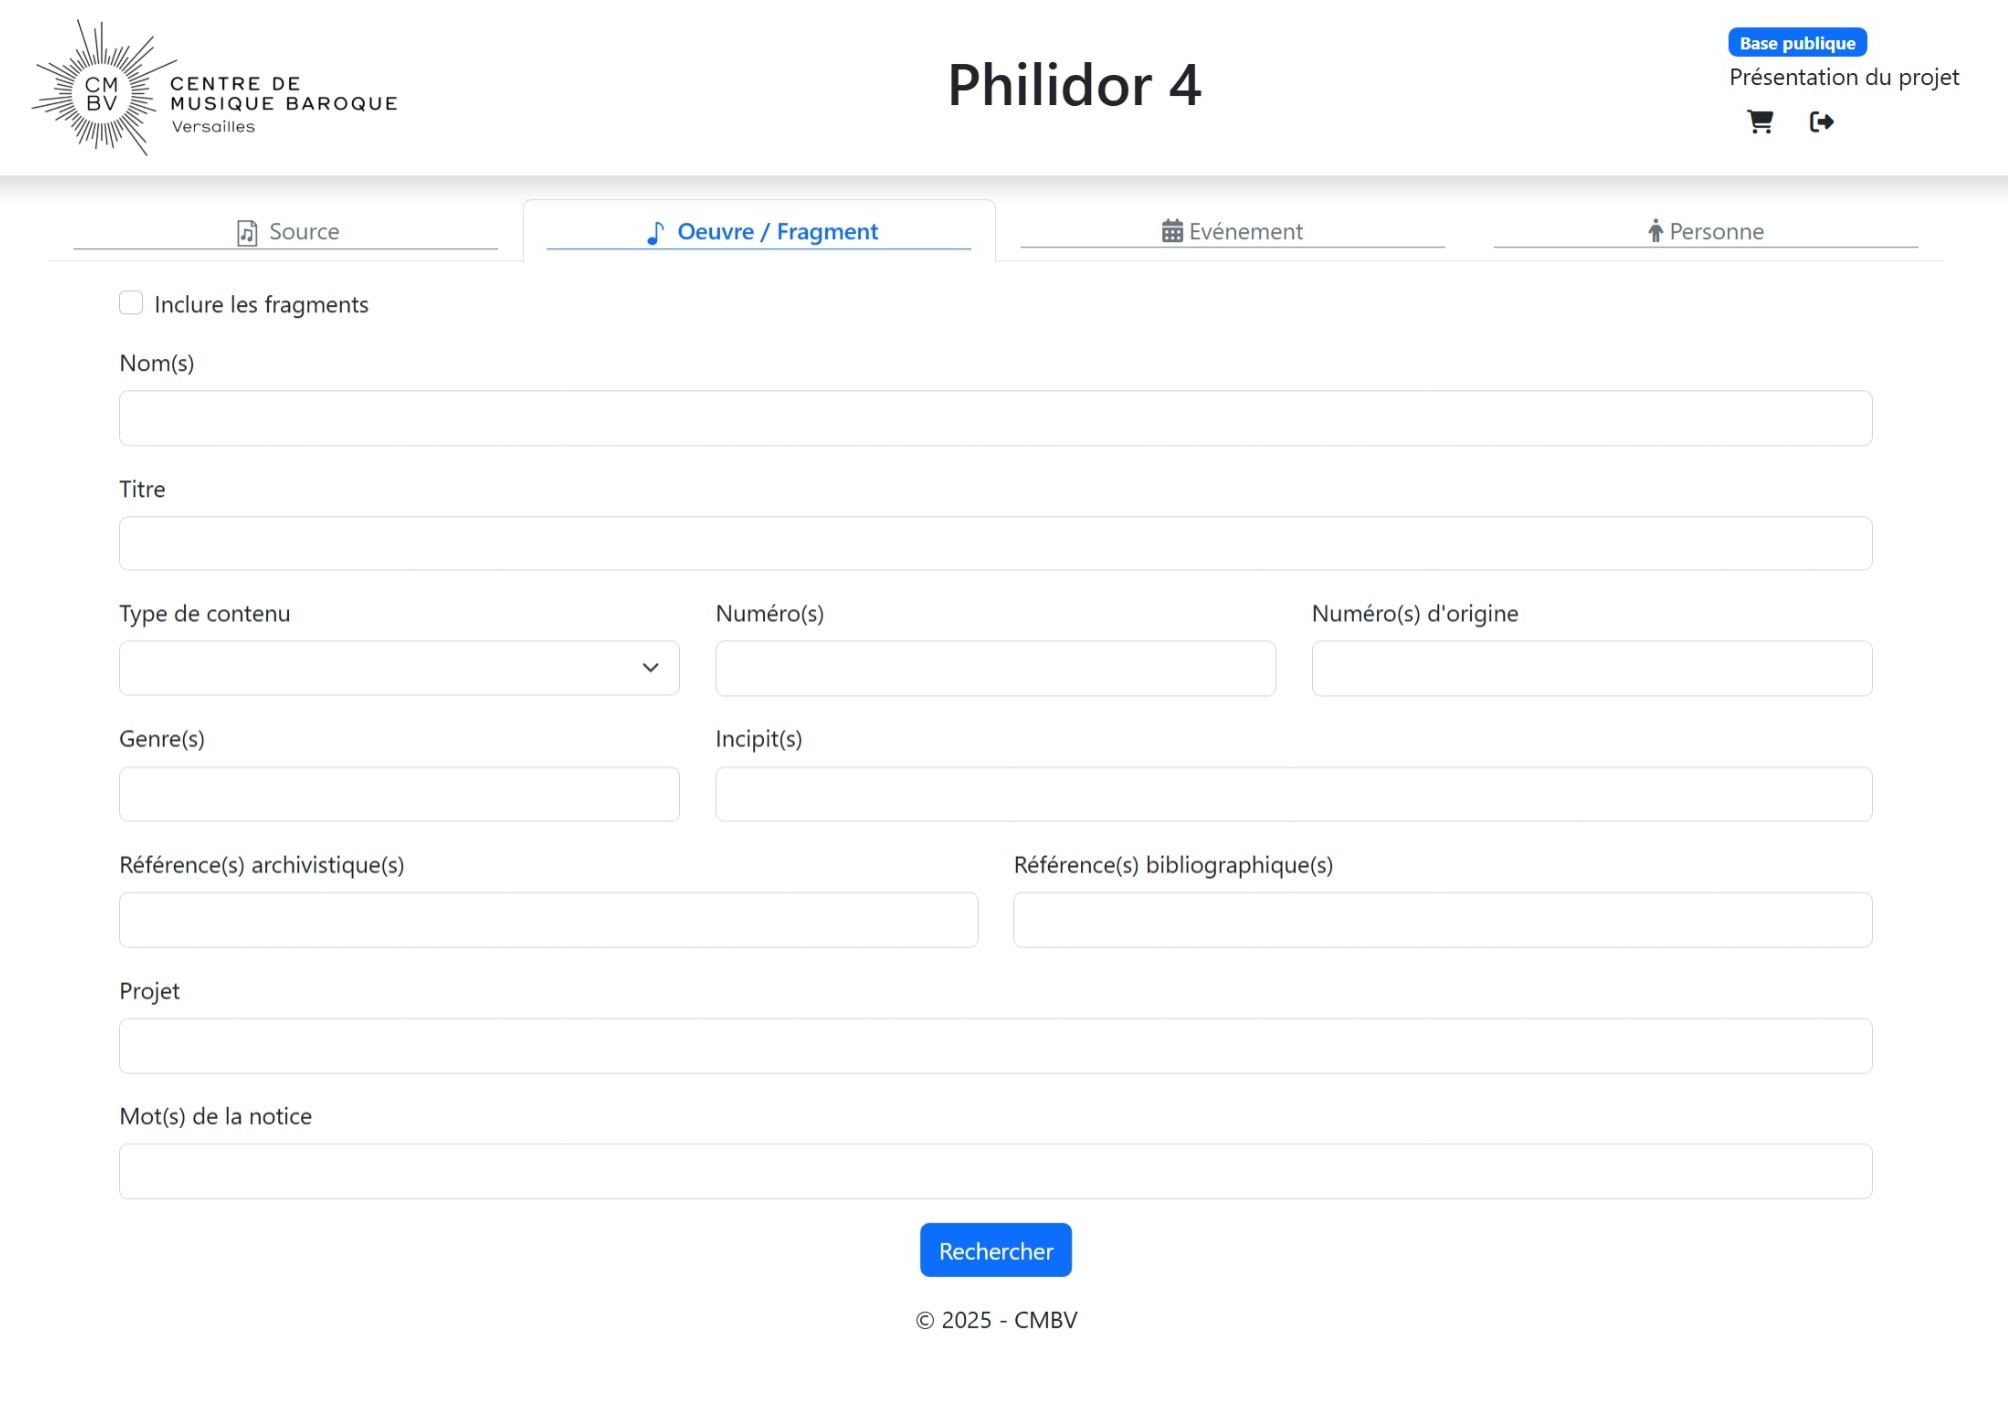
\includegraphics[width=\textwidth]{images/Capture_ecran_onglet_oeuvres_philidor4.jpeg}
\end{figure}

Cette distinction entre œuvres et fragments soulève des questions épistémologiques importantes, comme qu'est-ce qui constitue une œuvre complète ? Par exemple, un air d'opéra peut être un air détaché d'une pièce d'opéra --- l'opéra étant alors l'œuvre --- mais peut aussi être considéré comme une œuvre à part entière. Ces questions donnent lieu à de nombreux débats. Esteban Buch met en évidence que le concept d'\textquote{œuvre musicale} peut représenter un spectre assez large de phénomènes différents \footcite{buchRelireIngardenOntologie2013}.

D'autre part, le choix technique d'une case à cocher ne rend pas compte de la complexité de ces catégorisations, créant parfois de la confusion pour l'utilisateur. Certains utilisateurs passent à côté de cette case sans la voir. Ce faisant, ils ne profitent pas de cette fonctionnalité et n'ont pas accès à une partie du corpus, car ils en ignorent l'existence.

La base \textsc{Événement}, plus simple, privilégie les critères temporels et spatiaux, avec la possibilité de recherche textuelle libre dans l'ensemble des notices (cf. figure \ref{formulaire_evenement}). La simplicité du formulaire reflète la nature plus homogène de ce type de données, comparativement à l'hétérogénéité des sources ou œuvres.

\begin{figure}[h]
	\caption{Onglet de recherche pour la sous-base \textsc{Événement}} \label{formulaire_evenement}
	\centering
	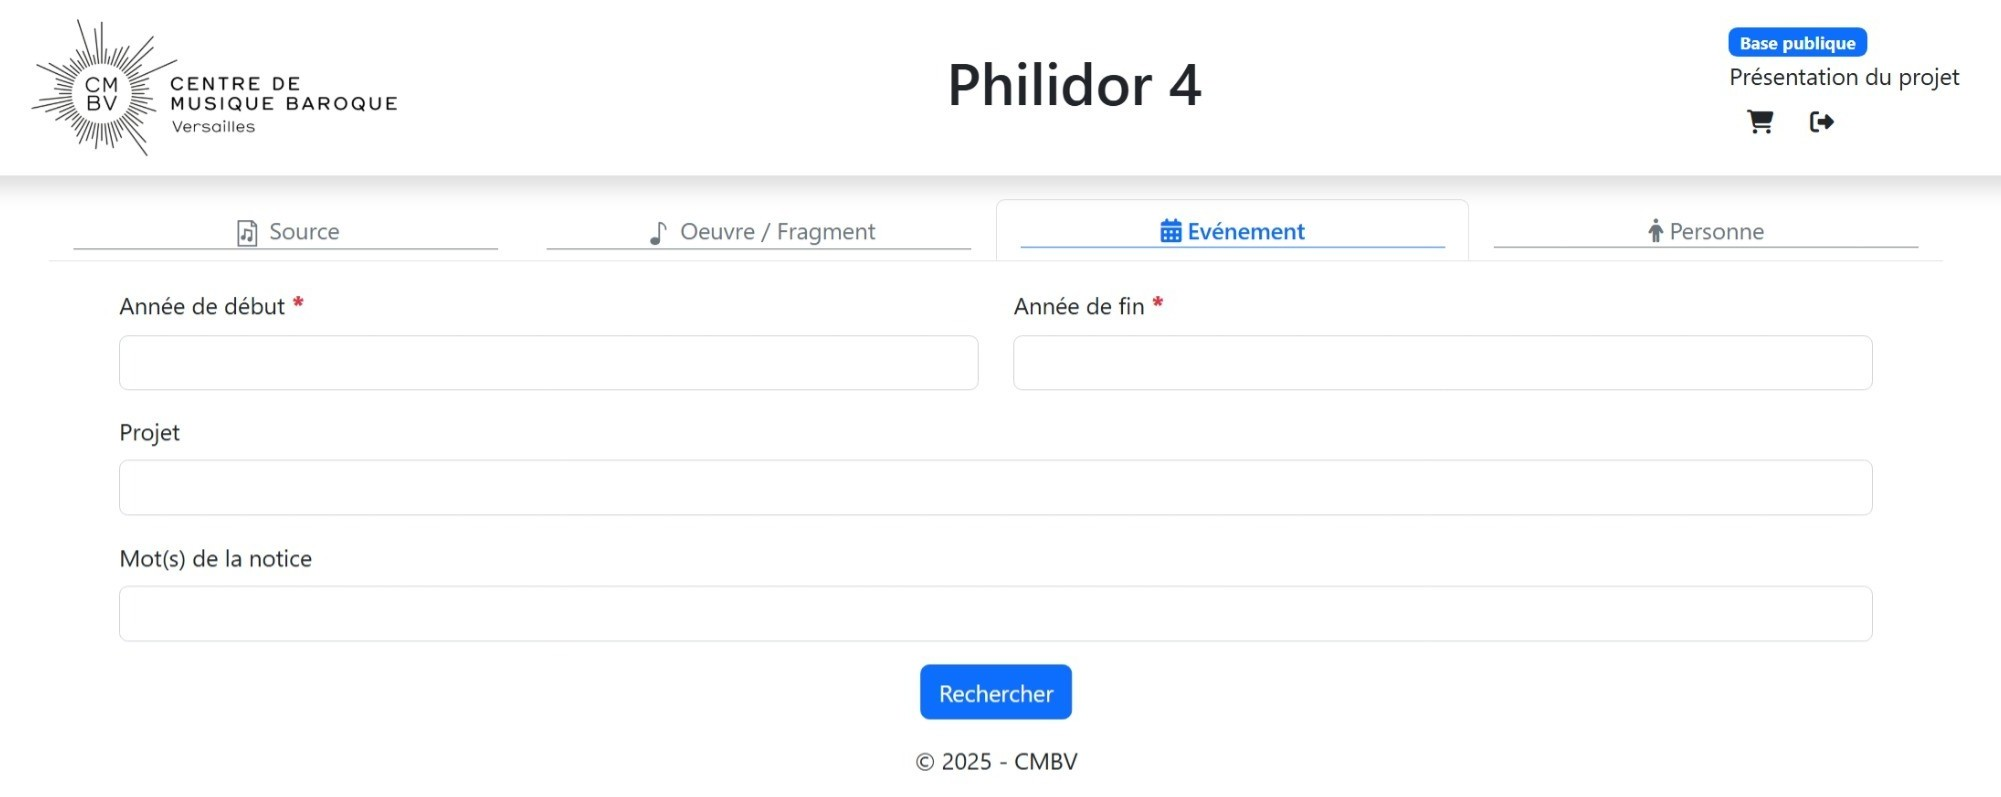
\includegraphics[width=\textwidth]{images/Capture_ecran_onglet_evenements_philidor4.jpeg}
\end{figure}

La base \textsc{Personne} (cf. figure \ref{formulaire_personne}) présente actuellement un périmètre limité aux musiciens romains (1570-1750), illustrant le caractère évolutif du projet. Cette spécialisation géographique et chronologique, si elle limite les possibilités de recherche, garantit la cohérence et la qualité des données \glslink{prosopographie}{prosopographique}s disponibles.

\begin{figure}[h]
	\caption{Onglet de recherche pour la sous-base \textsc{Personne}} \label{formulaire_personne}
	\centering
	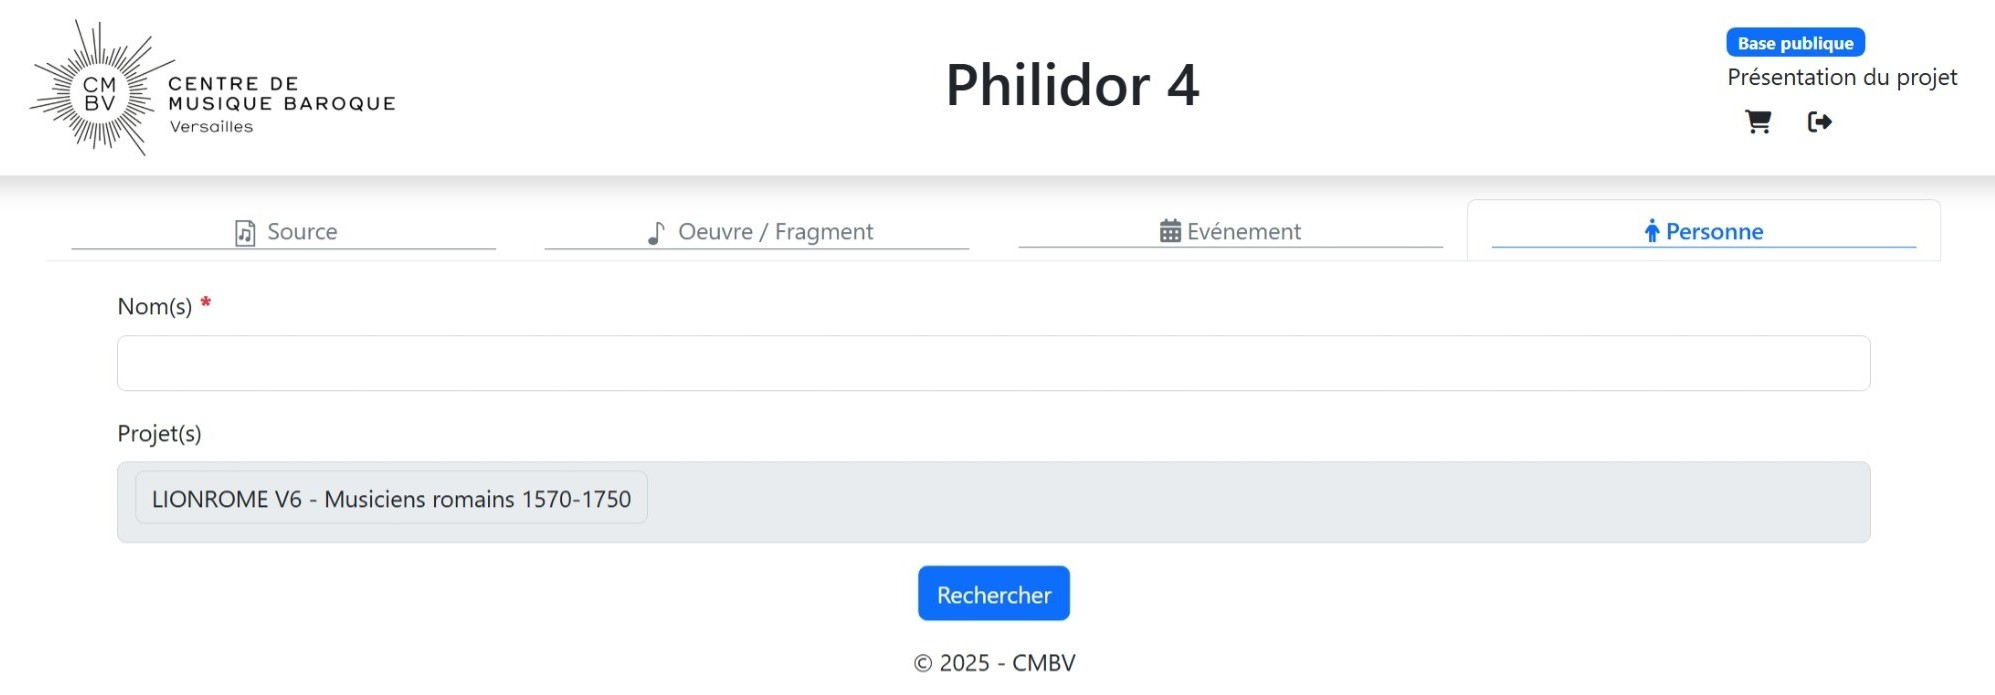
\includegraphics[width=\textwidth]{images/Capture_ecran_onglet_personnes_philidor4.jpeg}
\end{figure}

L'objectif idéal serait d'étendre cette couverture à toutes les personnes référencées dans les autres sous-bases en tant qu'autorité. Cela souligne l'ambition de constituer un référentiel \glslink{prosopographie}{prosopographique} exhaustif. Cette évolution transformerait qualitativement l'outil en permettant des recherches relationnelles et biographiques approfondies, croisant les différentes activités d'une même personne à travers les différents corpus.

\subsubsection{Fonctionnalités avancées et recherche par autorités}

La recherche par autorités est l'un des points forts du système. Le champ \textquote{Nom(s)}, présent dans trois des quatre sous-bases, propose une interface d'autocomplétion dynamique : la liste déroulante s'adapte en temps réel à la saisie, facilitant l'identification des personnes référencées. Cette fonctionnalité témoigne d'une conception orientée vers la normalisation des données d'autorité, enjeu central dans les bases de données. L'autocomplétion présente plusieurs avantages : elle réduit les erreurs de frappe, harmonise l'orthographe des noms propres, et révèle l'existence de formes variantes ou de personnes aux noms similaires. Cette assistance à la saisie améliore significativement la qualité des requêtes et la pertinence des résultats, particulièrement importante pour les noms d'époque aux graphies instables.

Les sous-bases \textsc{Source} et \textsc{Œuvre} offrent la gamme de critères la plus étendue, reflétant la complexité de la description des objets documentaires et musicaux. Cette richesse permet d'établir des liens entre des notices en les interrogeant selon des axes variés. La multiplicité des points d'entrée favorise les découvertes inattendues et les rapprochements novateurs, dimension essentielle de la recherche exploratoire\footcite{laurentguilloRapportMigrationAnciennes2022}.

\subsubsection{Présentation et exploitation des résultats}

Le format d'affichage est standardisé selon les informations disponibles dans les notices. Pour les œuvres et les fragments, le format est le suivant : \textbf{Numéro} - \textbf{titre} - \textbf{incipit} - \textbf{genre musical} - \textbf{genre du texte}. Cette uniformisation, si elle facilite le parcours rapide des résultats, appauvrit l'information disponible en première lecture. On remarque notamment que le compositeur des œuvres n'est pas mentionné ; or, certains textes comme celui du \textit{Magnificat} peuvent avoir été mis en musique par de nombreux compositeurs. Certaines notices apparaissent également vides comme on peut le voir sur la figure \ref{resultat_ercole}, faute de titres et de genre sur la notice.

\begin{figure}[h]
	\caption{Résultat de la recherche pour les œuvres du projet \textit{Bembo} avec \textquote{Ercole} dans le champ \textquote{Mot(s) de la notice}} \label{resultat_ercole}
	\centering
	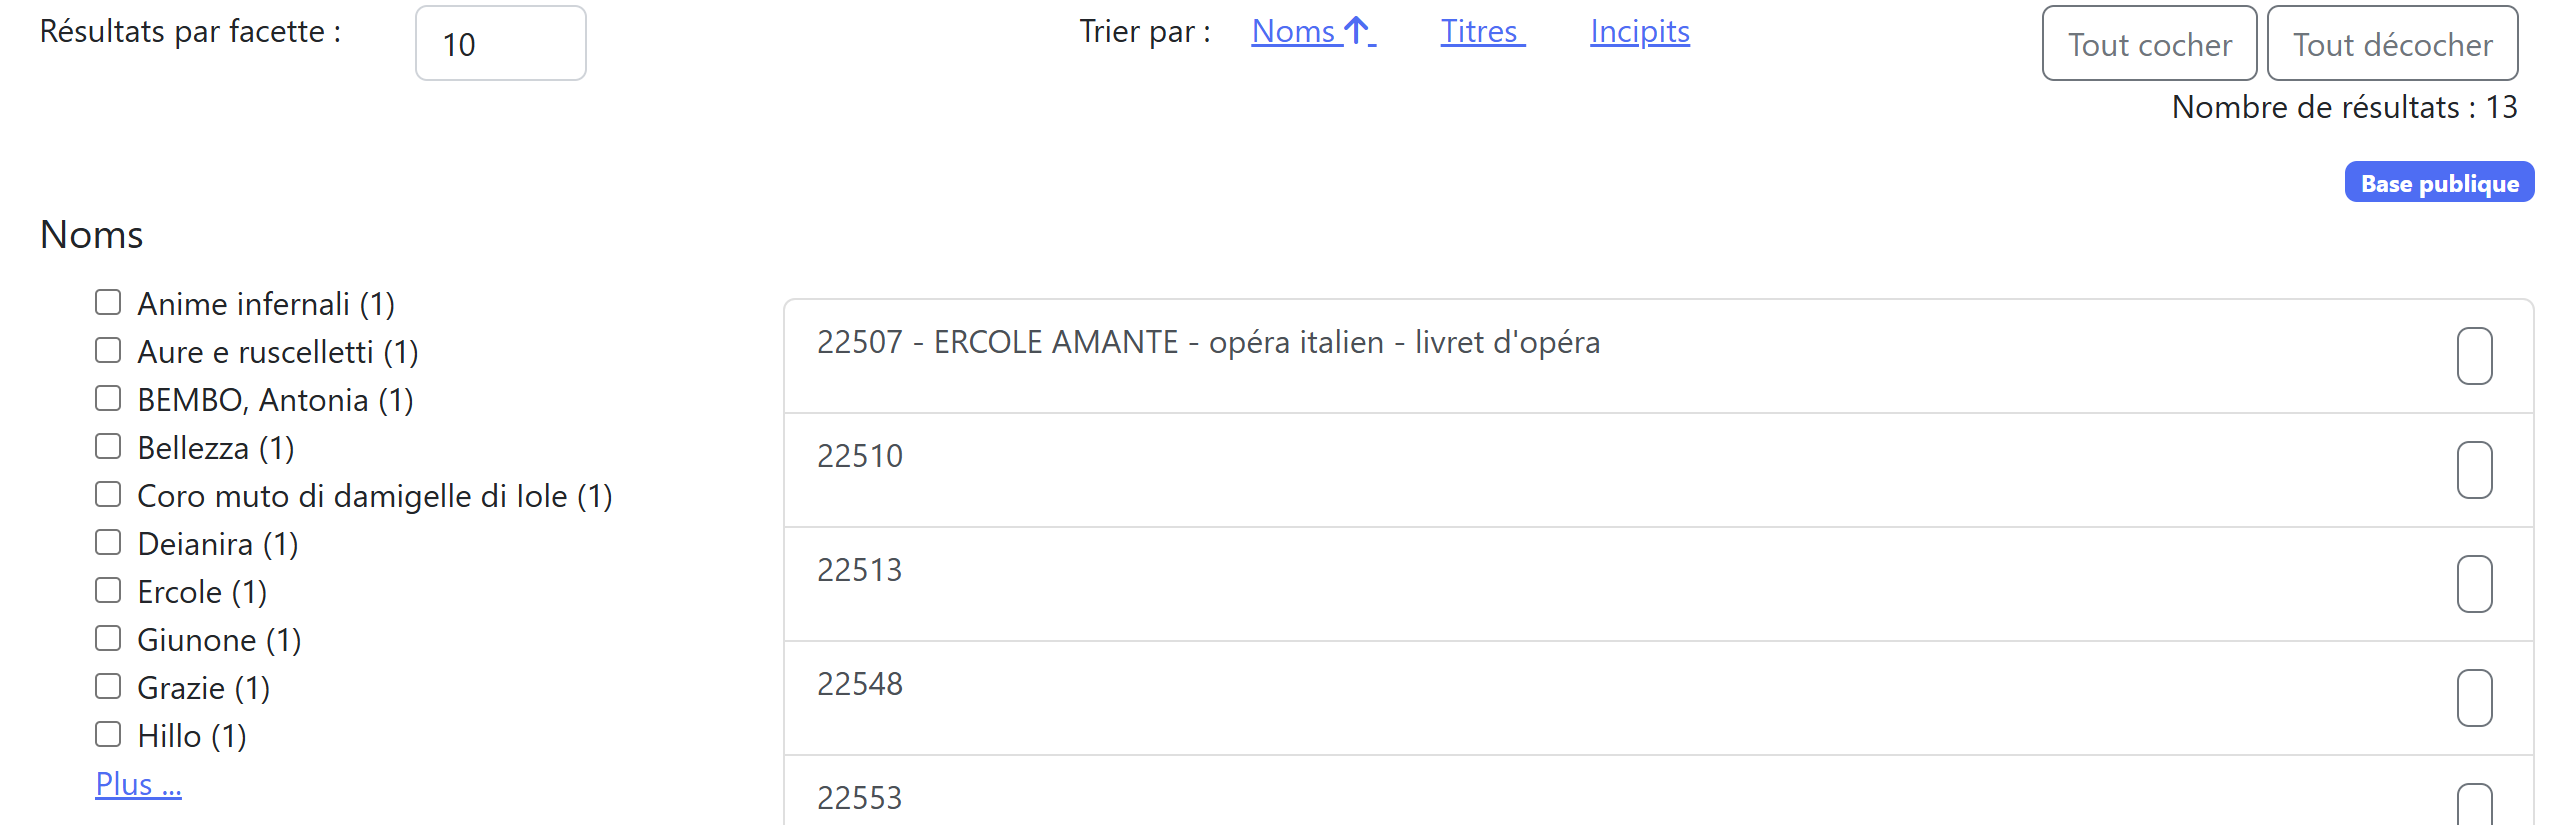
\includegraphics[width=\textwidth]{images/Capture_ecran_resultats_sans_titre.png}
\end{figure}

L'affichage des résultats suit une logique de raffinement progressif. Les facettes, positionnées en colonne gauche, permettent un filtrage a posteriori selon des critères variables : noms et titres pour les sources, noms, titres et incipits pour les œuvres, lieux et noms pour les événements et personnes. Cette approche par facettes facilite l'exploration des corpus volumineux. Ces informations, automatiquement générées à partir des résultats, constituent une forme d'analyse documentaire en temps réel, permettant à l'utilisateur d'évaluer la pertinence et l'exhaustivité de sa requête.

\begin{figure}[h]
	\caption{Résultat de la recherche pour les œuvres et les fragments du projet \textit{Bembo} triés par titre croissant} \label{resultat_bembo}
	\centering
	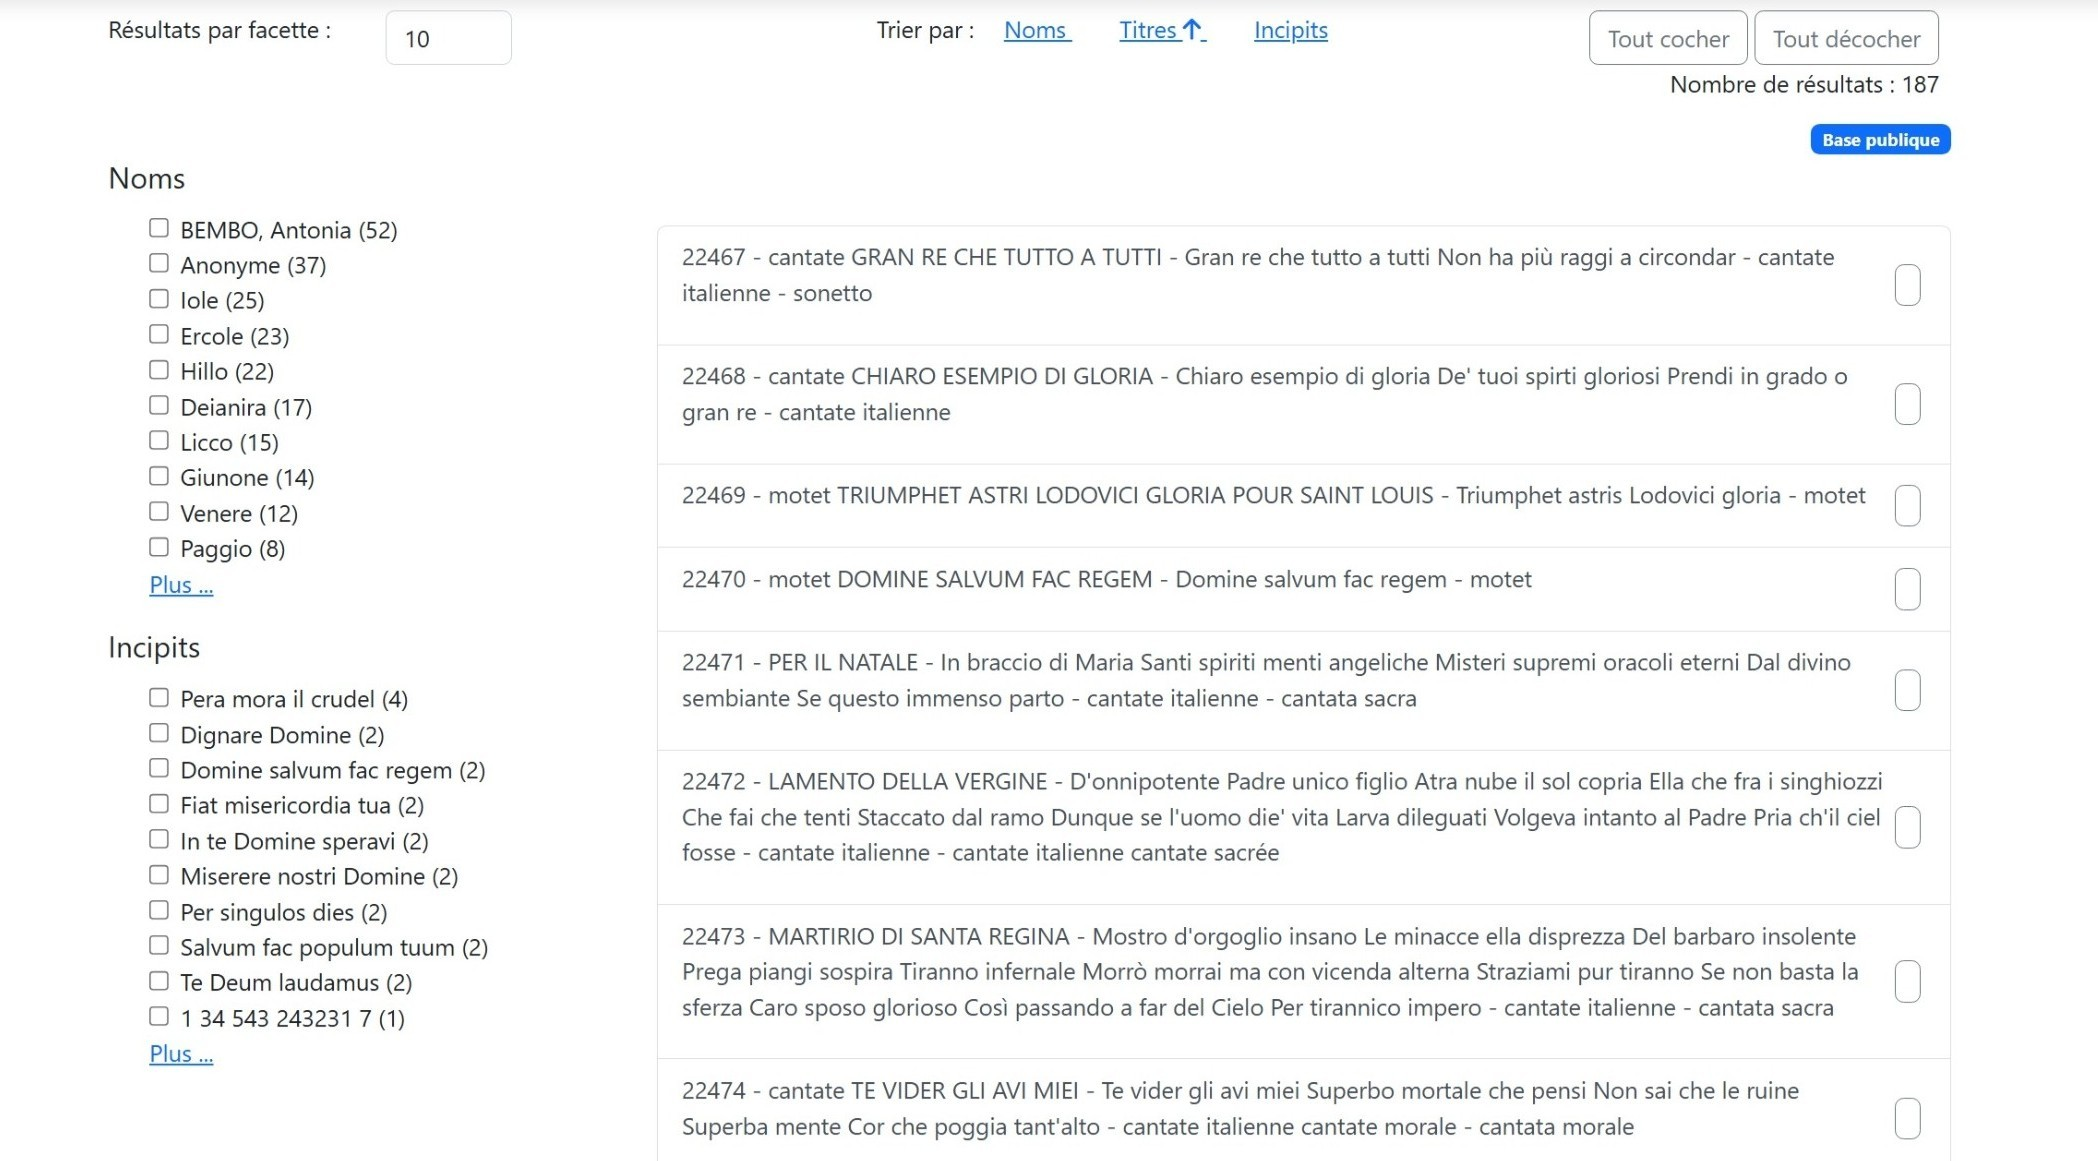
\includegraphics[width=\textwidth]{images/Capture_ecran_resultat_bembo_avec_frag_titre_croissant.jpeg}
\end{figure}

D'autre part, le système de tri révèle des dysfonctionnements : l'ordre alphabétique par titre n'est pas respecté, comme l'illustre la figure \ref{resultat_bembo} où les notices semblent trié par numéro. Cela compromet la lisibilité des résultats. Ces problèmes techniques, apparemment mineurs, affectent significativement l'expérience utilisateur, particulièrement lors de la consultation de corpus volumineux nécessitant un parcours ordonné.

\subsubsection{Limites ergonomiques et défis techniques}

Comme le souligne Ghislaine Chartron, \textquote{la découvrabilité désigne la capacité d’un contenu à être trouvé}\footcite{chartronEditionPublicationContenus2016}. Les processus de référencement et les \glslink{algorithmie}{algorithmes} de classement ont ainsi un poids considérable dans le domaine de l'accès à l'information\footcite{chartronEditionPublicationContenus2016}. Cependant, les rendre efficaces n'est pas forcement chose aisée. En effet, les algorithmes modernes sont d'une grande complexité, utilisant un grand nombre de variables et pouvant être composés d'ensembles d'algorithmes\footcite{richardDansBoiteNoire2018a}.

L'utilisation du moteur de recherche de \textit{Philidor~4} révèle des difficultés récurrentes : phénomènes de bruit (résultats non pertinents) et de silence (résultats manqués) qui compromettent l'efficacité des recherches. La recherche par titre présente des dysfonctionnements liés à la répartition des informations dans différents attributs selon la nature des objets décrits. Cette dernière, apparemment simple, révèle des tensions structurelles : une même information peut se trouver dans le champ \textquote{Œuvre}, \textquote{Titre-clé} ou encore \textquote{Titre-clé source} selon le type de notice. Ces anomalies s'expliquent par la complexité de la migration : les informations historiquement saisies dans des champs distincts selon les projets ont été harmonisées selon une logique nouvelle, créant parfois des inadéquations entre la structure des données et les attentes des utilisateurs.

Ces limites révèlent les tensions inhérentes aux bases de données hétérogènes : concilier la spécificité des descriptions avec l'unification des modes d'accès. La solution de contournement qui peut être utilisée est d'utiliser le champ \textquote{Mot(s) de la notice} pour la recherche par titre. Cela illustre l'écart entre la logique structurelle de la base et les attentes intuitives des utilisateurs. On peut citer l'exemple de l'opéra \textit{Ercole Amante} qui ne ressort pas dans les résultats lorsque l'on tape le titre dans le champ de recherche \textquote{Titre}, mais qui ressort au milieu de bruit si l'on utilise le champ \textquote{Mot(s) de la notice}.

Ces difficultés s'expliquent aussi par l'écart récurrent entre les intentions des concepteurs et les attentes réelles des utilisateurs. Comme le souligne Chevalier, \textquote{les utilisateurs ne lisent pas le Web, ils le parcourent}\footcite{chevalierChapitreErgonomieInterfaces2013}, ce qui rend les dysfonctionnements encore plus sensibles lorsqu'une recherche ne renvoie pas immédiatement des résultats pertinents.

L'ergonomie d'une interface ne dépend donc pas seulement de la richesse de la modélisation, mais aussi de sa capacité à limiter la charge cognitive des usagers\footcite{chevalierChapitreErgonomieInterfaces2013}. Une structuration trop rigide ou trop complexe accentue les risques de désorientation et freine la fluidité de l'exploration. Ces constats rejoignent l'idée que la variabilité des profils d'utilisateurs impose de concevoir des parcours de recherche souples, capables de s'adapter à des pratiques hétérogènes\footcite{chevalierChapitreErgonomieInterfaces2013}.

\subsection{Présentation des données : architecture informationnelle et affichage}

Présenter les données de manière claire et cohérente n'est pas évidente. Effectivement, il faut composer entre les aspects techniques et les attentes des utilisateurs.

\subsubsection{Architecture informationnelle : typologie fonctionnelle des champs}

L'architecture des notices s'articule autour de trois catégories fonctionnelles de champs, chacune répondant à des objectifs distincts et reflétant les différentes finalités de la base\footcite{BaseDonneesPHILIDOR42024}. Cette structuration tripartite constitue l'ossature conceptuelle qui organise l'ensemble de l'information disponible.

\paragraph{Les champs de gestion} assurent la traçabilité et l'\gls{interoperabilite} des données : auteur et date de saisie, état de validation, identifiants d'autorité externes (\gls{bnf}, \glslink{idref}{IDREF}, \gls{isni}, \glslink{viaf}{VIAF}), numérotations internes et historiques, rattachement aux projets, typologie du contenu. Ces métadonnées administratives constituent l'épine dorsale technique de la base.

\paragraph{Les champs descriptifs} portent l'information patrimoniale proprement dite : titres, adresses bibliographiques, arguments d'œuvres, descriptions de costumes et décors, discographies, éditions modernes, effectifs musicaux, événements biographiques, localisations géographiques, références archivistiques et bibliographiques. Cette couche descriptive traduit la richesse documentaire des sources primaires en données structurées.

\paragraph{Les champs d'indexation} opèrent une normalisation sémantique destinée à faciliter la recherche : vocabulaires contrôlés pour les fonctions, collectivités et genres, standardisation des dates et effectifs, incipits normalisés, mots-clés thématiques, titres-clés uniformisés. Cette dimension normative constitue la valeur ajoutée intellectuelle de la base, transformant la diversité des sources en corpus interrogeable.

\subsubsection{Modalités d'affichage et lisibilité}

En revanche, l'interface utilisateur ne reflète pas cette structuration conceptuelle : les informations s'affichent dans un format linéaire uniforme, en tant que succession de paragraphes associant intitulé de champ (en caractères gras) et contenu. Ce dernier peut être mis en page avec un certain nombre de sauts de ligne. Cette présentation \textquote{à plat} masque la hiérarchisation logique des données (cf. figure \ref{notice}) et peut désorienter l'utilisateur face à l'hétérogénéité apparente des informations.

\begin{center}
	\begin{figure}[p]
		\caption{Une notice d'une œuvre dans \textit{Philidor~4}} \label{notice}
		\centering
		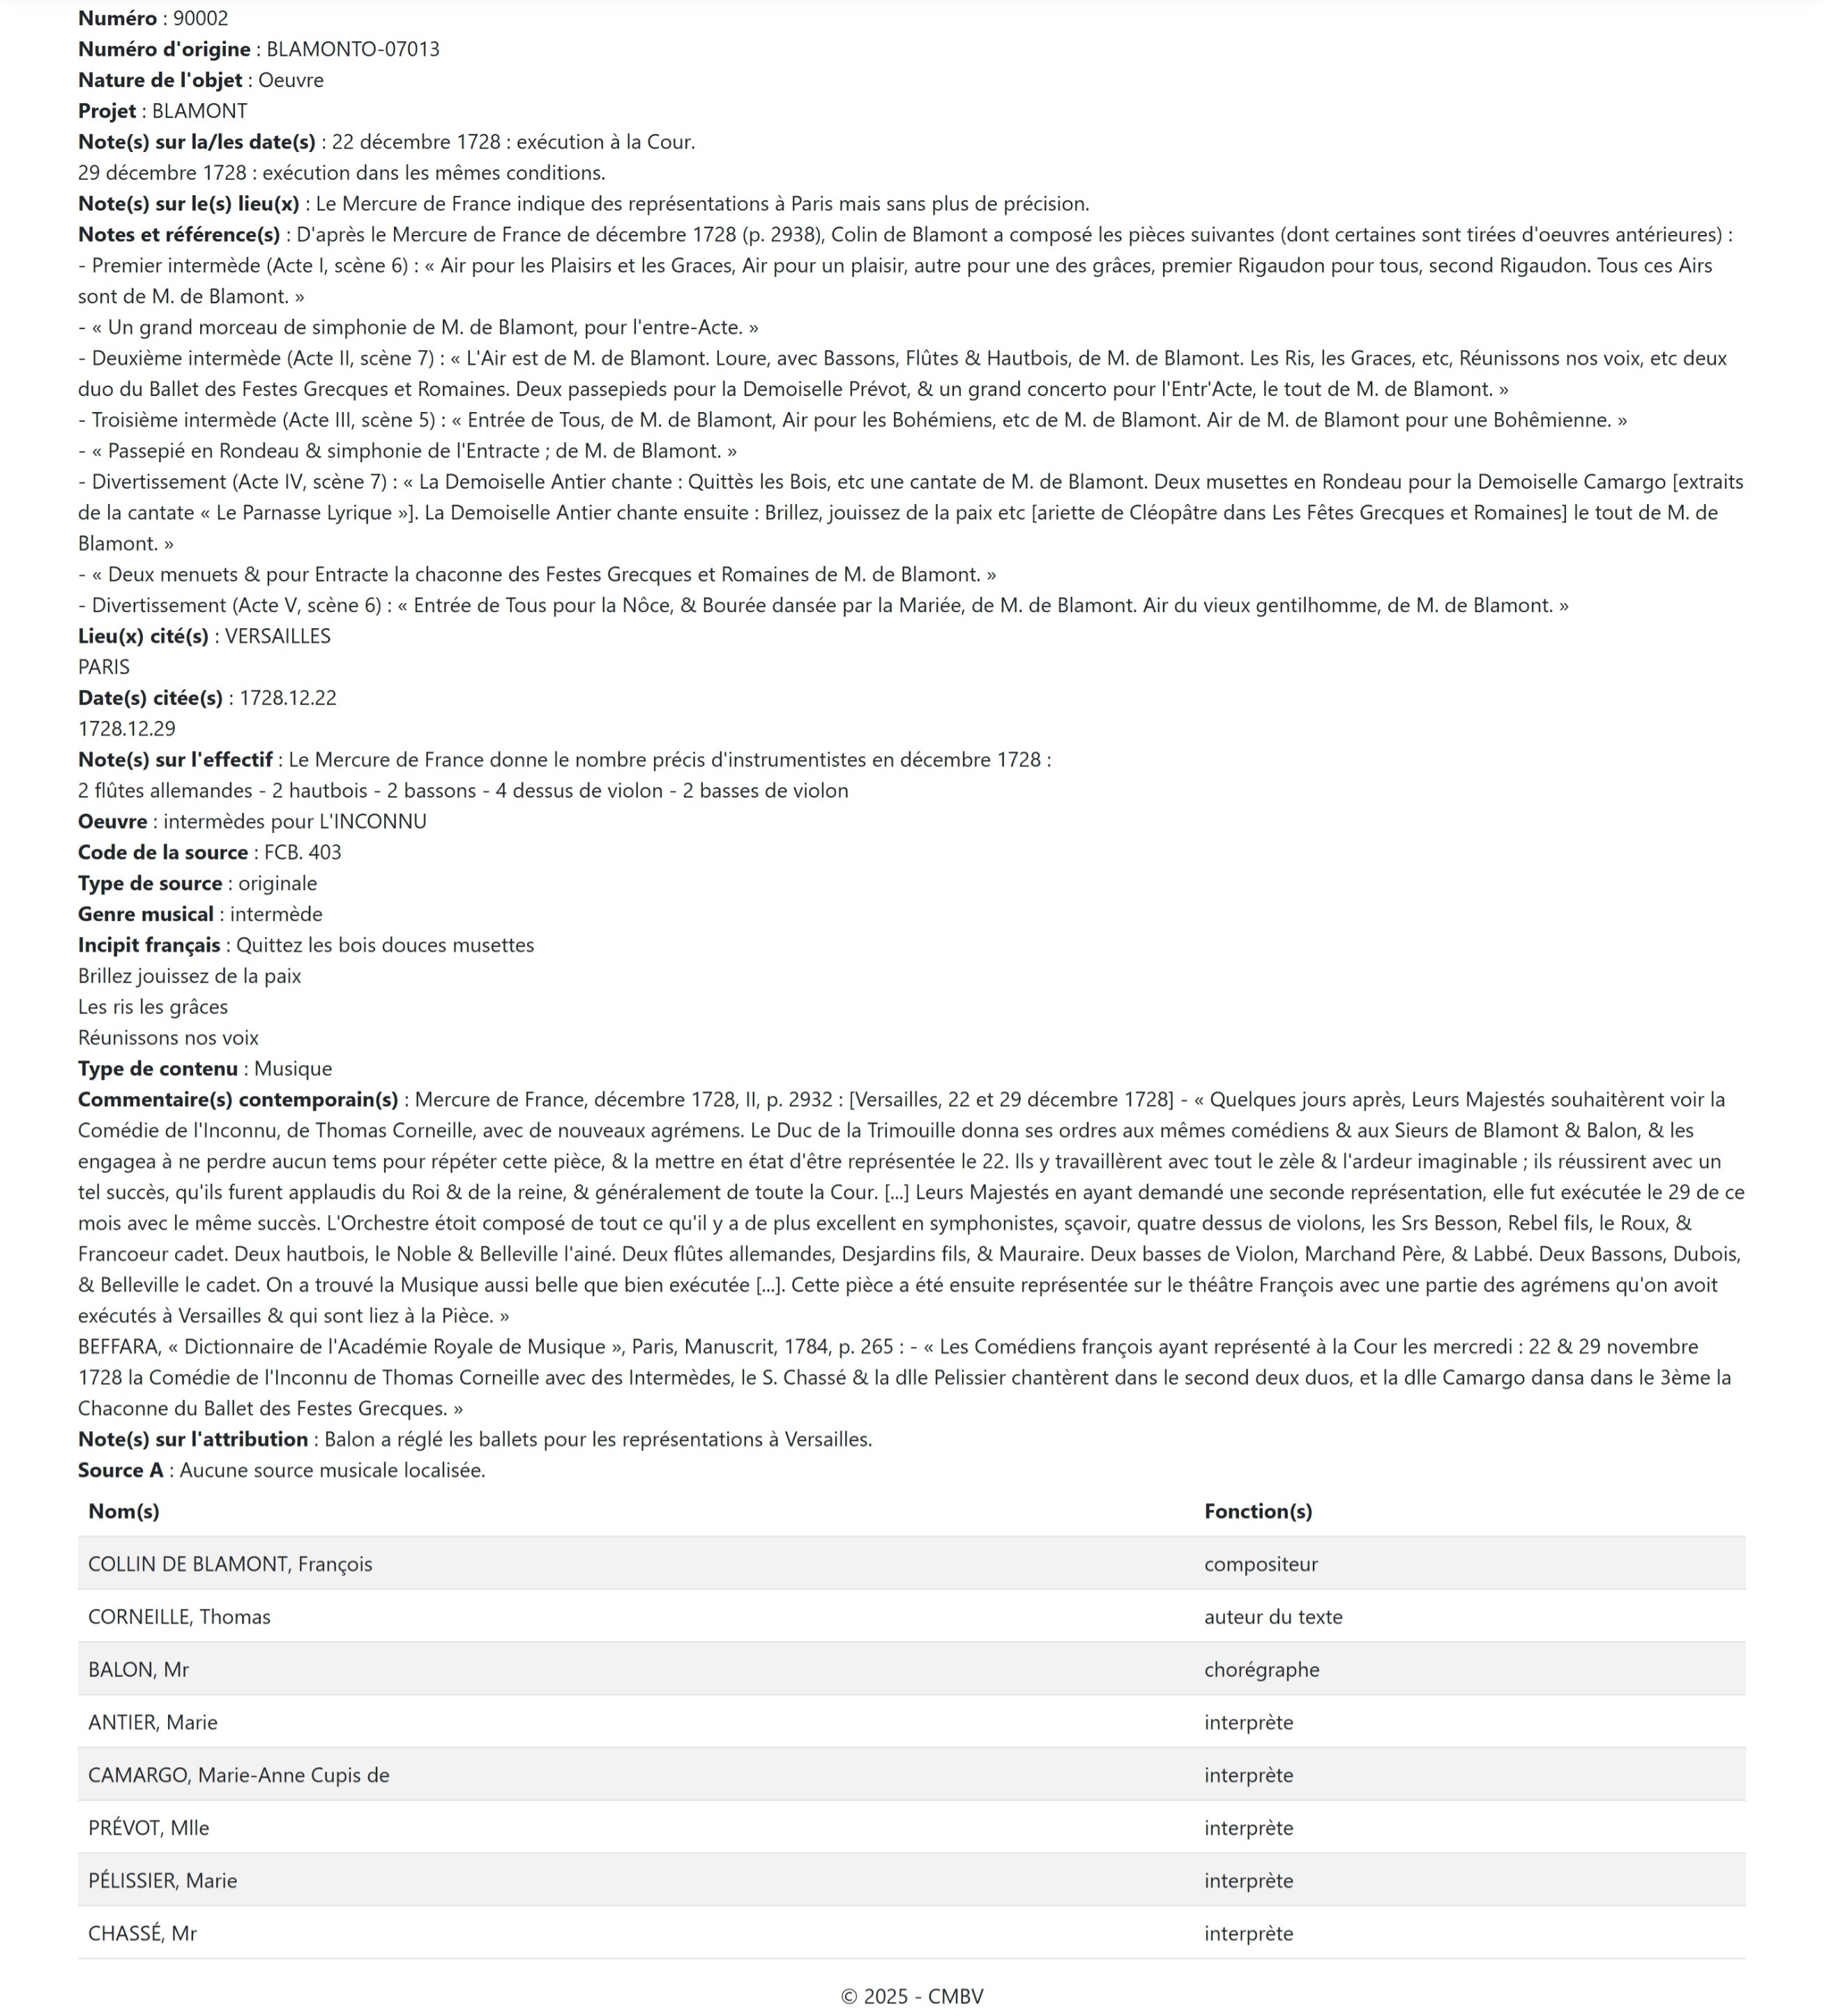
\includegraphics[width=\textwidth]{images/Capture_ecran_notice.jpeg}
	\end{figure}
\end{center}

Cette uniformisation de l'affichage, si elle simplifie la programmation, pose des questions ergonomiques importantes. L'absence de regroupement visuel selon les catégories fonctionnelles (gestion, description, indexation) complique la lecture et l'appropriation des notices, particulièrement pour les utilisateurs occasionnels peu familiers de la logique documentaire sous-jacente.

L'identification des titres illustre particulièrement les difficultés induites par cette structuration complexe. En effet, le titre n'est pas présent en haut de la notice, il faut donc le chercher. Selon la nature de la notice, l'information titre migre dans des champs distincts : \textquote{Œuvre} pour les œuvres complètes, \textquote{Genre et titre du fragment} pour les extraits comme l'illustre la figure \ref{notice_frag}, \textquote{Titre clé} ou \textquote{Titre clé source} pour les notices de la sous-base \textsc{Source}. Cette logique, cohérente du point de vue de la modélisation, génère une incertitude pour l'utilisateur qui doit \textquote{deviner} où chercher l'information principale.

\begin{center}
	\begin{figure}[h]
		\caption{Une notice d'un fragment dans \textit{Philidor~4}} \label{notice_frag}
		\centering
		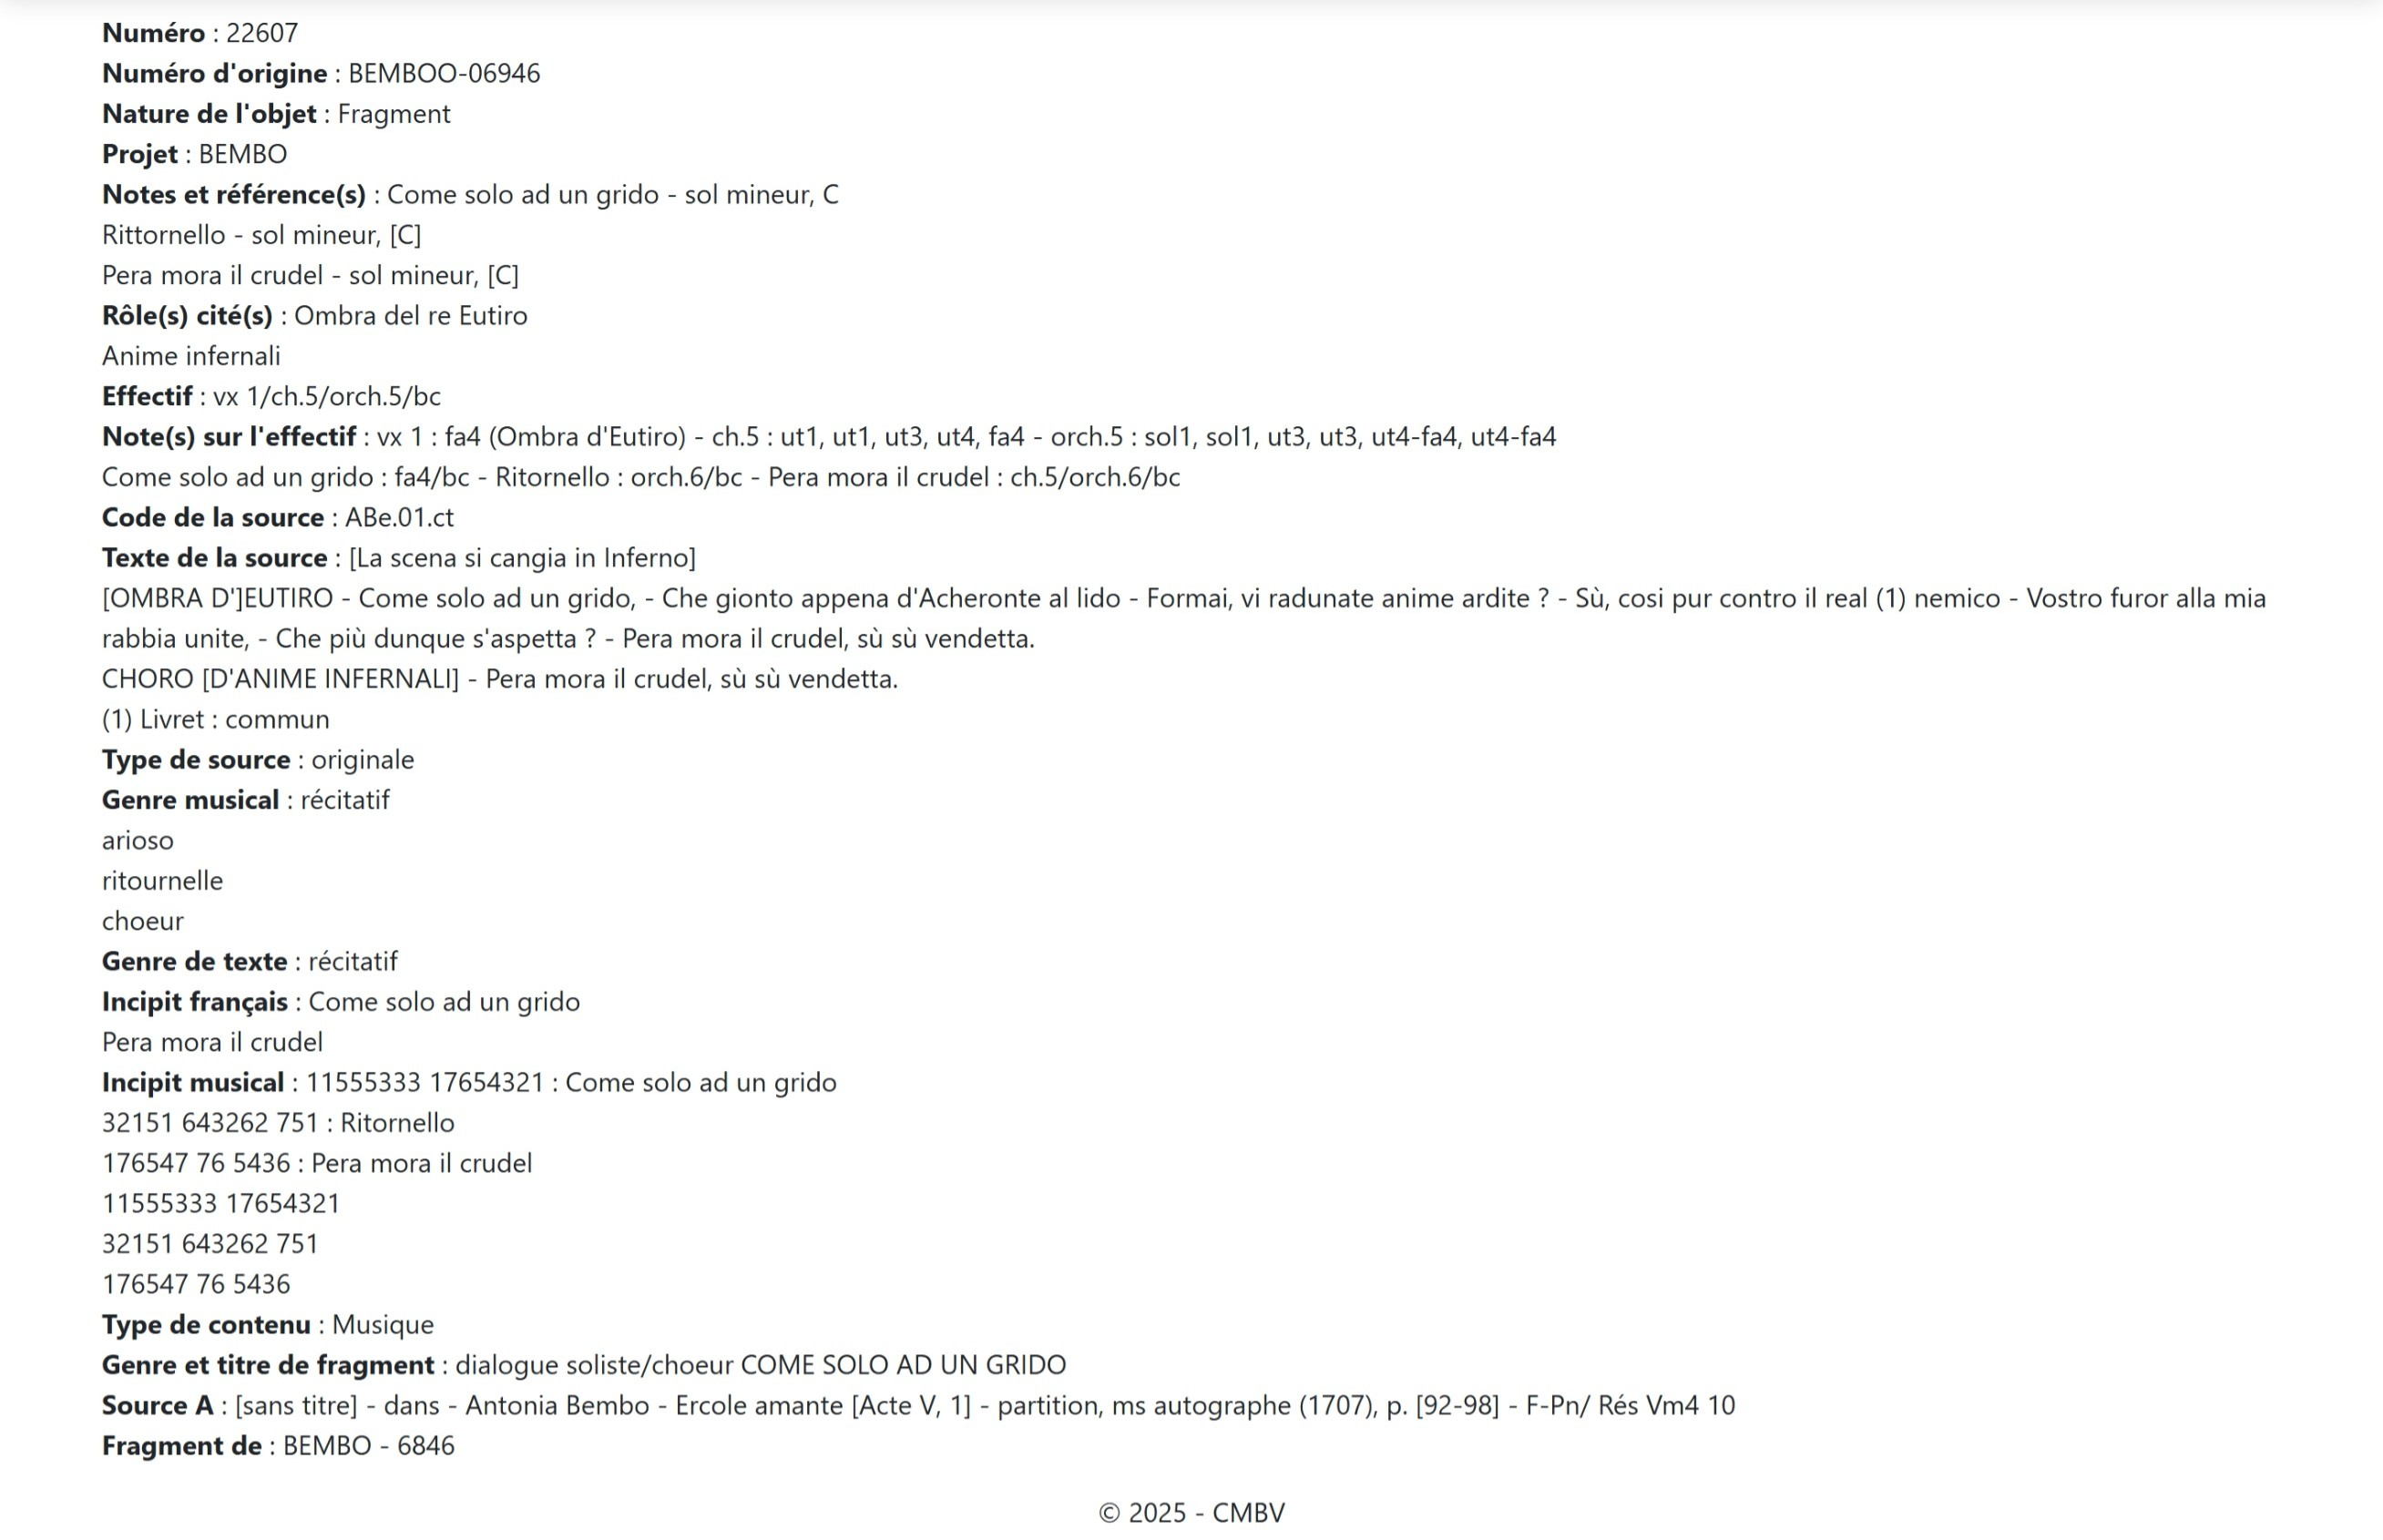
\includegraphics[width=\textwidth]{images/Capture_ecran_notice_frag.jpeg}
	\end{figure}
\end{center}

On note également l'exemple des champs \textquote{Note(s) sur la/les date(s)} et \textquote{Note(s) sur le(s) lieu(x)} qui apparaissent dans les premiers sur la notice, tandis que les champs \textquote{Date(s) citée(s)} et \textquote{Lieu(x) cité(s)} apparaissent bien plus bas. La hiérarchisation des champs n'étant pas claire, l'usager doit donc parcourir la notice avec beaucoup d'attention pour repérer les champs qui l'intéressent.

La gestion des fragments révèle d'autres incohérences. Les liens hiérarchiques entre œuvres et fragments ne sont pas reconstitués visuellement, remplacés par de simples listes de \textquote{numéros d'origine simplifiés} (cf. figure \ref{frag_ercole_amante}). Ces identifiants techniques (BEMBO au lieu de BEMBOO, absence du suffixe distinctif O pour \textquote{œuvre}) perdent leur signification mnémotechnique et compliquent la navigation entre notices liées.

\begin{figure}[h]
	\caption{Exemple de l'affichage des fragments pour l'opéra Ercole Amante d'Antonia Bembo} \label{frag_ercole_amante}
	\centering
	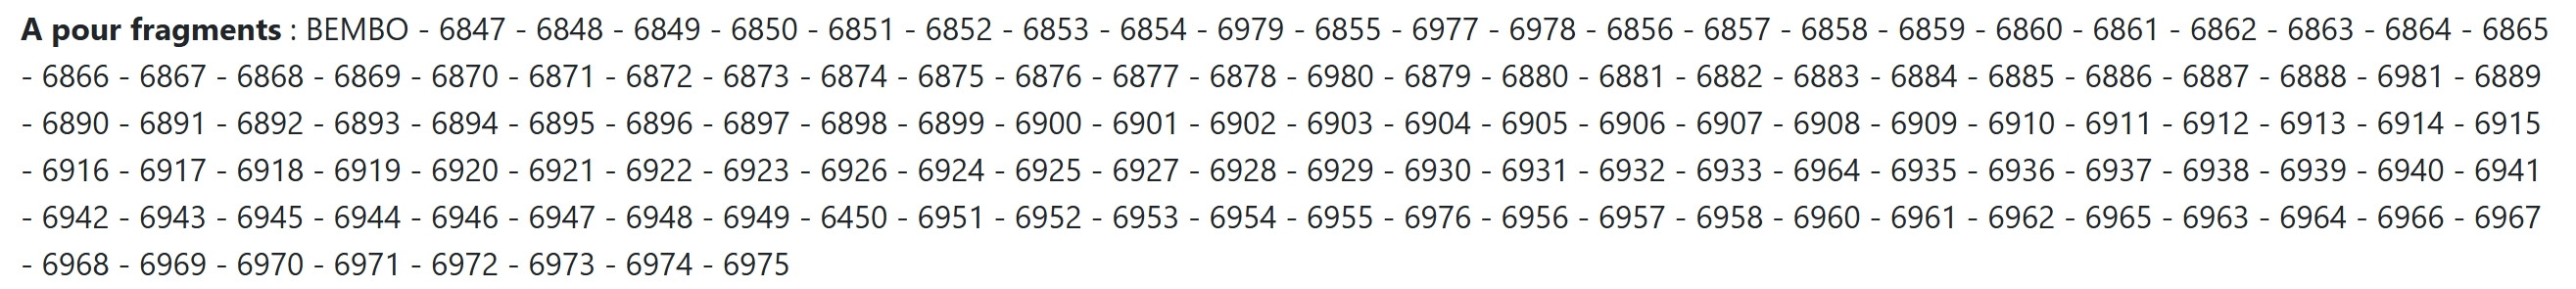
\includegraphics[width=\textwidth]{images/Capture_ecran_ex_frag.jpeg}
\end{figure}

Bien que MySQL permette la création de base de données relationnelle\footcite{duboisMySQLGuideOfficiel2004}, les relations qui ont pu être reconstitué n'ont donc pas été formalisé avec un système de clés primaire et étrangère permettant la navigation d'un objet à un autre.

Cette problématique de présentation révèle un enjeu fondamental des bases de données patrimoniales : concilier la complexité inhérente aux objets culturels avec les attentes de lisibilité des utilisateurs contemporains.

\subsection{Accessibilité et ouverture : entre barrières d'usage et enjeux d'\gls{interoperabilite}} \label{accessibilite_et_ouverture}

L'interface de \textit{Philidor~4} révèle une conception privilégiant la fonctionnalité technique au détriment de l'\gls{accessibilite} utilisateur. Cela peut s'expliquer par la volonté de rassembler toutes les données dans un système techniquement viable, même si l'ergonomie n'est pas parfaite, pour ensuite travailler sur l'\gls{accessibilite}.

\subsubsection{Barrières à l'appropriation et courbe d'apprentissage}

La multiplicité des onglets de recherche impose une certaine vigilance. Pour certain, dans la précipitation, cela implique une exploration par essai-erreur. Cela peut être décourageant pour les utilisateurs occasionnels. L'absence de parcours guidé --- tutoriels, aide contextuelle, ou même exemples de requêtes types --- contraint chaque nouvel utilisateur à reconstituer individuellement la logique du système. Le \gls{pdf} \textquote{\textsc{Philidor4} - Contenu et recherche} (cf. annexe \ref{philidor4-contenu-recherche}) donne une idée des champs et de leur contenu respectif ainsi que quelques astuces pour la recherche. Cependant, ce \gls{pdf} est téléchargeable uniquement sur l'interface de connexion à une session publique. Une fois connecté, il faut se déconnecter pour pouvoir y avoir de nouveau accès si on ne l'a pas téléchargé.

Le design purement fonctionnel, dépourvu d'éléments visuels engageants ou de parcours de découverte, engendre un risque, le fait de se décourager avant d'atteindre les ressources pertinentes. Contrairement aux interfaces contemporaines qui accompagnent l'utilisateur par des suggestions ou des parcours recommandés, \textit{Philidor~4} maintient une approche \textquote{experte} qui présuppose une connaissance préalable des enjeux musicologiques, et même de la structure de la base. 

De plus, l'interface, conçue pour les écrans d'ordinateur, s'adapte mal aux usages mobiles désormais majoritaires dans la consultation web. Or, une interface bien conçue est cruciale pour une bonne expérience utilisateur\footcite{gantierRetroingenierieWebdocumentaireFind2020}. On peut notamment citer les formulaires de recherche, dimensionnés pour des écrans larges, qui deviennent difficilement manipulables sur smartphones, excluant de fait une part significative des utilisateurs potentiels. Samuel Gantier et Antonin Jousse souligne que des problèmes d'utilisabilité peuvent inclure des difficultés de navigation, des superpositions d'éléments, ou l'impossibilité de contrôler le zoom\footcite{gantierRetroingenierieWebdocumentaireFind2020}. Dans le cas de \textit{Philidor~4}, un zoom s'active automatiquement lorsque l'on veut taper quelque chose dans un champ mais le zoom n'est pas pratique lorsqu'il s'agit d'un champ avec des valeurs prédéfinies à sélectionner.

\subsubsection{Formats d'export et réutilisation des données}

La fonctionnalité de \textit{panier} permet à l'usager de cocher les notices qu'il souhaite enregistrer depuis l'interface de recherche. Une fois les notices dans le panier, il est possible d'en retirer, de vider le panier ou d'exporter ce dernier.

La nature temporaire des paniers (liée à la session) limite cependant son utilité pour les recherches au long cours, fréquentes en recherche académique. Cette limitation technique contraint les utilisateurs à des stratégies de contournement peu pratiques : téléchargement systématique, captures d'écran, ou reconstitution manuelle des corpus lors de sessions ultérieures. L'absence de sauvegarde permanente traduit une conception de l'usage privilégiant les consultations ponctuelles plutôt que les projets de recherche étendus.

Par ailleurs, les fonctionnalités d'export de \textit{Philidor~4} révèlent une conception limitée de la réutilisation des données. Les trois formats proposés --- \gls{pdf}, \gls{xml}, email --- répondent à des besoins distincts mais présentent chacun des limitations importantes pour l'intégration dans les \textit{\glspl{workflow}} de recherche contemporains.

L'export \gls{pdf}, s'il permet une consultation hors ligne et une impression aisée, génère un document statique peu exploitable pour l'analyse ou la citation. Il imprime simplement chaque notice avec la même mise en forme que sur l'interface web, séparée par un saut de page de la notice suivante. La mise en forme automatique, fonctionnelle mais rudimentaire, ne rivalise donc pas avec les standards de présentation attendus dans les publications académiques. L'absence de génération automatique de références bibliographiques normalisées contraint par ailleurs les utilisateurs à reformater manuellement les données.

Le format \gls{xml}, théoriquement plus riche, est documenté par le \gls{pdf} \textquote{\textsc{Philidor4} - Contenu et recherche} qui précise l'ensemble des balises qui peuvent être présentes. Cependant, certaines balises sont mal orthographiées, car elles sont indiquées avec des caractères accentués, ce qui n'est pas le cas dans la réalité. La documentation présente aussi quelques lacunes. La balise \textit{nomFonction} n'est, en effet, pas décrite dans la documentation. Elle comporte normalement des éléments \textit{item} avec des attribut \textit{key} indiquant la forme normalisée du nom d'une personne. Dans certain cas, au lieu de trouver le nom de la personne dans la valeur de l'attribut \textit{key}, l'attribut \textit{key} n'existe pas et on a une balise portant le nom de la personne ou une balise anonyme comme dans l'exemple suivant :

\begin{codeblock}{xml}
<nomsFonctions>
    <item key="DANIELIS, Daniel">compositeur</item>
    <item key="CHARPENTIER, Marc-Antoine">compositeur</item>
    <item key="LALLOUETTE, Jean-François [attr. possible]">compositeur</item>
    <item key="BERNIER, Nicolas [attr. poss.]">compositeur</item>
    <Anonyme>compositeur</Anonyme>
    <TREVISO>compositeur</TREVISO>
    <item key="ZUMBACH, Lotharius">compositeur</item>
    <item key="GAULTIER, Pierre">compositeur</item>
</nomsFonctions>
\end{codeblock}

Ces complexités techniques limitent l'exploitation de l'export par les utilisateurs avancés qui souhaiteraient intégrer les données dans leurs propres outils d'analyse. L'absence d'\gls{api} publique accentue cette fermeture : aucun moissonnage automatique n'est possible.

L'incompatibilité avec les gestionnaires de références bibliographiques (Zotero, Mendeley, EndNote) constitue un obstacle majeur à l'intégration dans les pratiques académiques. Cette lacune contraint les chercheurs à des saisies manuelles chronophages et génératrices d'erreurs, réduisant l'attractivité de la ressource face à des alternatives mieux intégrées.

\subsubsection{Positionnement dans l'écosystème numérique patrimonial}

L'analyse de l'\gls{interoperabilite} de \textit{Philidor~4} révèle un positionnement en retrait par rapport aux standards contemporains du \textit{\gls{web-semantique}}. Bien que la base intègre des identifiants d'autorité externes (\gls{bnf}, \glslink{idref}{IDREF}, \gls{isni}, \glslink{viaf}{VIAF}), leur exploitation demeure limitée : aucun lien hypertexte ne permet de naviguer vers ces référentiels, et l'information reste purement indicative.

Cette sous-exploitation des standards d'autorité contraste avec les pratiques développées par les bibliothèques numériques contemporaines, qui transforment ces identifiants en véritables pivots de navigation inter-bases. L'absence de liens sortants vers les notices équivalentes dans \gls{rism}, la \gls{bnf} ou d'autres ressources musicologiques limite les possibilités d'enrichissement documentaire et d'exploration transversale.

La conformité aux standards de métadonnées demeure également problématique. Si les champs de \textit{Philidor~4} peuvent théoriquement être mappés vers des schémas comme Dublin Core ou les recommandations \gls{tei}, aucune exposition de ces données selon ces formats n'est proposée. \textit{Philidor~4} n'est donc pas présent dans des agrégateurs comme Europeana ou les portails nationaux du patrimoine numérique. Cette base demeure donc pour le moment une ressource isolée, accessible uniquement par consultation directe.

Cette situation pose des questions importantes sur la pérennité et la visibilité de la ressource. Dans un contexte où la découvrabilité des contenus passe de plus en plus par l'agrégation et l'\gls{interoperabilite}, l'isolement technique de \textit{Philidor~4} risque de limiter sa diffusion et son impact scientifique. La richesse des contenus est indéniable, mais se trouve partiellement neutralisée par une interface difficilement exploitable.

\section*{Conclusion du chapitre}

L’analyse de \textit{Philidor~4} met en lumière la complexité d’une base de données patrimoniale à l’ère des refontes technologiques. Héritière de trois décennies d’accumulations documentaires et de choix techniques successifs, cette nouvelle version illustre à la fois la continuité d’un projet fondateur et la nécessité d’une restructuration profonde. La genèse du projet, marquée par une mobilisation collective et la difficile consolidation de données hétérogènes, révèle l’importance des arbitrages techniques et humains dans la construction d’un tel outil.

L’examen de son architecture modulaire, organisée autour des entités \textsc{Source}, \textsc{Œuvre}, \textsc{Événement} et \textsc{Personne}, souligne la pertinence conceptuelle de cette modélisation tout en mettant en évidence ses limites pratiques. Si cette structuration offre une vision riche et hiérarchisée du patrimoine musical, elle engendre également des frictions d’usage, perceptibles dans la répartition inégale des données et les difficultés de navigation rencontrées par certains utilisateurs.

L’évaluation ergonomique enfin montre un outil puissant mais encore marqué par des tensions entre exhaustivité scientifique et \gls{accessibilite} fonctionnelle. Les performances du moteur de recherche, la qualité d’affichage des notices et la navigation interne constituent autant d’indicateurs de ces équilibres fragiles.

Ces constats soulignent les enjeux stratégiques de l'évolution technique des bases de données patrimoniales : comment concilier spécificité disciplinaire et standards d'\gls{interoperabilite} ? Comment maintenir la cohérence scientifique tout en s'adaptant aux exigences techniques contemporaines ?

Ce chapitre révèle ainsi l’ambivalence de \textit{Philidor~4} : projet innovant dans sa conception, mais confronté à des défis d’appropriation et de pérennité. Cela ouvre sur une réflexion plus large concernant les alternatives éditoriales et les perspectives de valorisation des données, qui seront abordées dans le chapitre suivant.